\documentclass[a4paper,ruledheader]{abnt}
\usepackage[brazil]{babel}
\usepackage[utf8]{inputenc}
\usepackage[pdftex]{graphicx}
\usepackage{latexsym}
\usepackage{psfrag}
\usepackage[section]{placeins}
\usepackage{float}
\usepackage[hidelinks]{hyperref}
\usepackage{morefloats}
\usepackage{afterpage}
\usepackage{supertabular}
\usepackage{longtable}
\usepackage[center]{caption}
\usepackage[export]{adjustbox} % loads also graphicx
\usepackage[]{times} %mesmo que Times New Roman
\usepackage{setspace} % espacamento entre linhas
\setstretch{1.5}% padrao 1.5 de espacamento entre linhas
\usepackage[titles]{tocloft} %Pacote para alinhar Sumarios
\setlength{\cftchapindent}{1.0cm}       % ajusta identação dos capítulos no sumário
\setlength{\cftsecindent}{1.0cm}      % ajusta identação das seções no sumário
\setlength{\cftsubsecindent}{1.0cm}     % ajusta identação das subseções no sumário
\usepackage{chngcntr}
\counterwithout{figure}{chapter}
\counterwithout{table}{chapter}

\renewcommand{\cftfigpresnum}{Figura ~ }
\renewcommand{\cfttabpresnum}{Tabela ~ }

\renewcommand{\cftfigaftersnumb}{- }
\renewcommand{\cfttabaftersnumb}{- }

\newlength{\mylenf}
\settowidth{\mylenf}{\cftfigpresnum}
\setlength{\cftfignumwidth}{\dimexpr\mylenf+0.8em}
\setlength{\cfttabnumwidth}{\dimexpr\mylenf+0.8em}
\renewcommand{\familydefault}{\sfdefault}

\setcounter{tocdepth}{4}
\DeclareGraphicsExtensions{.pdf,.jpg,.png}

\def\changemargin#1#2{\list{}{\rightmargin#2\leftmargin#1}\item[]}
\let\endchangemargin=\endlist


\renewcommand{\ABNTsectionfontsize}{\flushleft\large\normalfont} %Altera o tamanho da fonte do sub-capitulo
\renewcommand{\ABNTsubsectionfontsize}{\flushleft\large\normalfont} %Altera o tamanho da fonte do sub-capitulo
\renewcommand{\ABNTchaptersize}{\large} %Altera o tamanho do titulo do capitulo



\begin{document}

\onehalfspacing %Espaçamento de 1.5

\graphicspath{{./images/}}%Estrutura básica do documento - Gerados por Template

\include{capa}
\include{folharosto}
\include{fichaCatalografica}
\include{folhaaprovacao}

%Gerados por conversão de documentos
\include{Resumo}
\include{Abstract}
\include{Dedicatoria}
%\include{Agradecimentos}
%\include{Epigrafe}
%Estrutura básica do documento - fim


\listoffigures
\listoftables
\tableofcontents

%Gerados por conversão de documentos
\include{Introducao}
\chapter{REVIS\~AO BIBLIOGR\'AFICA}

\bigskip

{
Durante o processo de desenvolvimento do TCC pesquisamos diversos softwares que s\~ao utilizados para o desenvolvimento
da documenta\c{c}\~ao de TCC a fim de ter o\ conhecimento sobre essas ferramentas, suas vantagens e desvantagens em
rela\c{c}\~ao ao desenvolvimento do TCC.}

{
As principais ferramentas utilizadas para desenvolvimento da documenta\c{c}\~ao do TCC s\~ao editores de texto WYSIWYG
(What you see is what you get, em portugu\^es ``O que voc\^e v\^e \'e o que voc\^e obt\'em'') como o~Microsoft Word que
diferente do {\LaTeX} possibilita que o documento que est\'a sendo criado possa ser editado e visualizado ao mesmo
tempo com suas altera\c{c}\~oes, por meio de atalhos que s\~ao selecionados pelo mouse\ ou atalhos, enquanto no
{\LaTeX} todo desenvolvimento do documento \'e feito por meio de c\'odigos que s\~ao interpretados e apresentados
visualmente ao usu\'ario apenas ap\'os a convers\~ao do documento para PDF ou algum outro formato pr\'e estabelecido. A
grande desvantagem de editores WYSIWYG \'e a dificuldade de formata\c{c}\~ao de documentos muito extensos e de
abordagem cient\'ifica, nos quais \'e exigida uma formata\c{c}\~ao padronizada e cheia de detalhes. Outra desvantagem
\'e na cria\c{c}\~ao e formata\c{c}\~ao de f\'ormulas matem\'aticas complexas\ que s\~ao muito comuns em documentos
cient\'ificos.}

{
Por esses motivos, muitas universidades levaram a exigir que os alunos utilizassem o {\LaTeX} para o desenvolvimento do
TCC, pois ele possui f\'acil formata\c{c}\~ao de qualquer tipo de texto e \'e um programa padr\~ao que\ existe h\'a
anos e n\~ao varia muito a cada nova vers\~ao al\'em de ser gratuito.}

{
Notamos que hoje, o melhor programa que permite o desenvolvimento de um TCC dentro de todas as normas ABNT e todas as
funcionalidades exigidas para isso \'e o {\LaTeX}, por\'em ele n\~ao \'e um\ programa intuitivo e de f\'acil
aprendizagem, principalmente para pessoas que n\~ao tem grande familiaridade com computa\c{c}\~ao.}

{
Em cada universidade a utiliza\c{c}\~ao das normas ABNT para formata\c{c}\~ao de trabalhos acad\^emicos \'e feita de
forma diferente e seguindo como base o documento ``Manual de Apresenta\c{c}\~ao para Trabalhos Acad\^emicos'' (TIMB\'O,
2013) desenvolvido pela Universidade Metodista de S\~ao Paulo, notamos a complexidade das normas e a grande\ quantidade
de cuidados que devem ser tomados pelos alunos para fazer uma documenta\c{c}\~ao corretamente. Usaremos os requisitos
deste documento como base para desenvolver o nosso software que intermediar\'a a intera\c{c}\~ao do aluno que
desenvolve o TCC com o {\LaTeX} e\ auxiliar\'a na formata\c{c}\~ao deste documento segundo as normas ABNT adotadas pela
UMESP.}


null
\chapter[REFERENCIAL TE\'ORICO]{ REFERENCIAL TE\'ORICO}

\bigskip

{
Durante o desenvolvimento do nosso projeto, utilizamos de algumas ferramentas de apoio ao desenvolvimento adequado ao
nosso tipo software, entre elas {\LaTeX},\ NetBeans IDE, APIs Java como Writer2Latex e \ JLR (Java Latex Report),
Tamb\'em utilizamos a metodologia Extreme Programming (XP). Neste cap\'itulo falaremos sobre cada uma dessas
ferramentas e metodologias.}


\bigskip

\section[XP {}-- EXTREME PROGRAMMING]{ XP -- EXTREME PROGRAMMING}

\bigskip

{
O Extreme Programming (XP)\ foi criado em 1997 por Kent Beck. ``A Extreme Programming (XP) \'e uma metodologia \'agil
para equipes pequenas e m\'edias que desenvolvem software baseado em requisitos vagos e que se modificam rapidamente''
(BECK, 2000).}

{
O XP visa garantir a satisfa\c{c}\~ao do cliente, enfatizando o desenvolvimento \'agil do projeto para o cumprimento das
estimativas e vem ocupando espa\c{c}o consider\'avel no mercado, que antes que antes era dominado por metodologias
tradicionais, como RUP -- Rational Unified Process.}

{
Este subcap\'itulo tem como objetivo fazer uma breve apresenta\c{c}\~ao dessa metodologia, seus valores e algumas de
suas pr\'aticas para justificar a utiliza\c{c}\~ao da mesma nesse projeto, evitando uma abordagem detalhada e
desnecess\'aria ao objetivo do projeto.}


\bigskip

{
VALORES XP}


\bigskip

{
{}``Metas\ individuais de curto prazo frequentemente entram em conflito com metas s\'ocias de longo prazo. As sociedades
aprenderam a lidar com esse problema desenvolvendo um conjunto de valores a serem compartilhados'' (BECK, 2000).
Extreme Programming possui cinco valores a partir dos quais s\~ao desenvolvidas todas as suas pr\'aticas.}


\bigskip

{
Esses s\~ao os cinco valores de XP:}

\liststyleLFOi
\begin{itemize}
\item {
\textrm{\textbf{Comunica\c{c}\~ao:}}\textrm{\ deve ser priorizado o di\'alogo presencial que melhora o entendimento
tanto entre cliente e desenvolvedor quanto dentro da pr\'opria equipe de desenvolvimento;}}
\item {
\textrm{\textbf{Simplicidade:}}\textrm{\ desenvolver apenas o que \'e essencial ao software evita que se produza algo
que n\~ao utilizado. Vale mais a pena adicionar modifica\c{c}\~oes a desenvolver c\'odigos in\'uteis;}}
\item {
\textrm{\textbf{Feedback:}}\textrm{\ quanto mais cedo for identificada a necessidade de mudan\c{c}as mais barato ser\'a
para o desenvolvedor e para o cliente aplica-las. Feedback constante permite a r\'apida identifica\c{c}\~ao de
poss\'iveis erros e da necessidade de mudan\c{c}as ou melhorias no software;}}
\item {
\textrm{\textbf{Respeito:}}\textrm{\ todos devem ser respeitados igualmente dentro e\ fora da equipe, pois todos
contribuem com o desenvolvimento. Todo o tipo de experi\^encia e conhecimento deve ser respeitado;}}
\item {
\textrm{\textbf{Coragem:}}\textrm{\ \'e necess\'aria para estar preparado para as constantes mudan\c{c}as que podem
ocorrer em um projeto de software, bem como para aplicar todos os valores de XP.}}
\end{itemize}

\bigskip

{
Pr\'aticas XP}


\bigskip

{
Cada uma das pr\'aticas de Extreme Programming visa atender um ou mais dos valores citados acima e n\~ao possuem nenhum
valor se n\~ao forem usadas buscando atender esses valores. Cada pr\'atica aplicada separadamente gera benef\'icios ao
projeto, mas a utiliza\c{c}\~ao de v\'arias pr\'aticas em conjunto pode-se notar um ganho de benef\'icios muito maior.}


\bigskip

{
Listaremos a seguir algumas pr\'aticas de XP que foram adotadas por essa equipe com uma breve descri\c{c}\~ao das
mesmas:}

\liststyleLFOii
\begin{itemize}
\item {
\textrm{\textbf{Cliente Presente:}}\textrm{\ o cliente faz parte da equipe do desenvolvimento de software e \'e
presen\c{c}a constante nesse processo, fornecendo feedback com a maior frequ\^encia poss\'ivel;}}
\item {
\textrm{\textbf{Jogo do Planejamento:}}\textrm{\ planejamento \'e uma atividade cont\'inua desempenhada durante todo o
projeto, esta\ postura admite que ao longo do projeto as prioridades e necessidades do cliente sofrem constantes
mudan\c{c}as, portanto o planejamento deve acompanhar essas mudan\c{c}as;}}
\item {
\textrm{\textbf{C\'odigo Coletivo:}}\textrm{\ todo o desenvolvedor tem\ acesso a todas as partes do c\'odigo
(inclusive\ aquelas que ele n\~ao programou) e podem fazer qualquer altera\c{c}\~ao sem ter que pedir permiss\~ao,
desde que haja necessidade de tal altera\c{c}\~ao;}}
\item {
\textrm{\textbf{Integra\c{c}\~ao Cont\'inua:\ }}\textrm{\'e feita constantemente a integra\c{c}\~ao do c\'odigo
produzido ao restante do sistema\ assegurando, ao final de cada integra\c{c}\~ao, a consist\^encia da base de
c\'odigo.}}
\item {
\textrm{\textbf{Ritmo Sustent\'avel:}}\textrm{\ recomenda que os membros da equipe trabalhem oito horas por dia e evitem
ao m\'aximo a utiliza\c{c}\~ao de horas-extras de trabalho.}}
\item {
\textrm{\textbf{Projeto Simples:}}\textrm{\ {}``o sistema deve ser projetado da maneira mais simples o poss\'ivel em
qualquer momento. A complexidade desnecess\'aria \'e removida assim que for descoberta'' (BECK,2000).}}
\end{itemize}
{
O usu\'ario de XP n\~ao tem a obriga\c{c}\~ao de aplicar todas as suas pr\'aticas, mas apenas aquelas que se adequarem
as necessidades do projeto.}


\bigskip

\subsection[Por que utilizamos XP]{ Por que utilizamos XP}

\bigskip

{
Decidimos aplicar XP devido a sua flexibilidade para com poss\'iveis mudan\c{c}as no decorrer do projeto e a
possibilidade de escolher e adaptar as pr\'aticas de XP as necessidades de nosso projeto e as restri\c{c}\~oes de nossa
equipe.}

{
Possu\'iamos tamb\'em um grande interesse, pessoal e profissional, em conhecer, aprender e aplicar essa metodologia que
vem ganhando espa\c{c}o no mercado de desenvolvimento de software.}


\bigskip

\section[LaTeX]{ {\LaTeX}}

\bigskip

{
{}``LATEX \'e um sistema para formata\c{c}\~ao de textos de documentos. Sua primeira vers\~ao amplamente dispon\'ivel,
misteriosamente numerada 2.09, apareceu em 1985{\textquotedbl} (LAMPORT, 1995)}

{
O {\LaTeX} \'e um pacote de macros para desenvolver e gerar documentos para impress\~ao com alta qualidade
tipogr\'afica, criado por Leslie Lamport e mantido por Frank\ Mittelbach atualmente, podendo ser utilizado um layout
profissional predefinido. O seu desenvolvimento usou o TeX como motor de formata\c{c}\~ao.}

{
TeX \'e um software da onde se originou o LaTex, foi desenvolvido por Donald E. Knuth que come\c{c}ou a escrev\^e-lo em
1977, \'epoca em que editoras gr\'aficas come\c{c}aram a utilizar equipamentos digitais para impress\~ao.}

{
Segundo Knuth (1984) ao ``preparar um manuscrito em formato TEX, voc\^e estar\'a dizendo a um computador exatamente como
o manuscrito deve ser transformado em p\'aginas cuja qualidade aparenta ser tipogr\'afica''.}

{
\textrm{Os caracteres T, E, X no nome derivam respectivamente das letras gregas tau, \'epsilon, e chi, como o nome do
TeX deriva do grego\ }\textrm{\textit{$\tau \text{\textgreek{'e}}\chi \nu \eta $}}\textrm{\ (habilidade, arte,
t\'ecnica) a sua pron\'uncia correta\ }\textrm{seria ``t\'ec''. J\'a a primeira s\'ilaba do nome se pronuncia
exatamente igual \`a palavra inglesa lay sendo a pronuncia correta para {\LaTeX} \'e ``lei-t\'ec''.}}


\bigskip

\subsection[Benef\'icios do Latex]{ Benef\'icios do Latex}

\bigskip

{
\textrm{Para o usu\'ario comum, que n\~ao conhece ou apenas ouviu falar do Latex, imediatamente deve se perguntar,
``esse \'e mais um\ processador de texto, mas porque devo usar?''. Alguns pontos para essa pergunta.}}


\bigskip

\liststyleLFOiii
\begin{itemize}
\item {
\textrm{Devido aos seus layouts padronizados, os textos nele baseado possuem uma apar\^encia de texto de gr\'afica;}}
\item {
O Latex e totalmente gratuito e pode funcionar em quase todas as\ plataformas;}
\item {
Produ\c{c}\~ao de textos estruturados;}
\item {
N\~ao \'e necess\'ario montar um layout para uso personalizado, o usu\'ario precisa apenas conhecer alguns comandos que
estruturam o documento;}
\item {
A constru\c{c}\~ao de f\'ormulas matem\'aticas, tabelas, refer\^encias, rodap\'es, \'indices no {\LaTeX} \'e totalmente
facilitado;}
\item {
O padr\~ao Latex \'e amplamente usado pela comunidade acad\^emica e cient\'ifica, sendo em alguns casos obrigat\'orio o
seu uso em trabalhos acad\^emicos.}
\end{itemize}

\bigskip

\subsection[Por que utilizamos LaTeX]{ Por que utilizamos {\LaTeX}}

\bigskip

{
Devido aos benef\'icios j\'a citados, o {\LaTeX} \'e muito\ utilizado em Universidades e Empresas de m\'edio e grande
porte para o desenvolvimento de relat\'orios, monografias, artigos e demais documentos que requerem um alto n\'ivel de
padroniza\c{c}\~ao.}

{
Observamos que o desenvolvimento do TCC demanda muito tempo dos alunos\ e a necessidade de aprender uma tecnologia
desconhecida para a maioria dos alunos apenas para desenvolver a documenta\c{c}\~ao do TCC limitava o tempo de trabalho
dos mesmos.}

{
Neste trabalho temos como objetivo principal desenvolver um software que intermediasse\ a intera\c{c}\~ao entre um aluno
que esteja desenvolvendo um TCC e o {\LaTeX}, tornando o processo de desenvolvimento do TCC mais intuitivo e isentando
o aluno da necessidade de aprender {\LaTeX} para desenvolver um TCC, com nosso programa sendo o instrumento para a\ sua
documenta\c{c}\~ao final.}


\bigskip

\section[AS CLASSES ABNTeX E ABNTeX2]{ AS CLASSES ABNTeX E ABNTeX2}

\bigskip

{
\textrm{O {\LaTeX}, usado amplamente pela comunidade acad\^emica para produ\c{c}\~ao de textos matem\'aticos e
cient\'ificos, n\~ao possu\'ia uma classe que se adaptasse a ABNT (Associa\c{c}\~ao Brasileira de Normas T\'ecnicas),
em 2001\ nasceu o projeto para adequa\c{c}\~ao do {\LaTeX} \`as normas ABNT, originando o pacote de macros chamado
abnTeX, que auxilia na adequa\c{c}\~ao da documenta\c{c}\~ao dos trabalhos acad\^emicos feitos com {\LaTeX} \`as normas
da ABNT. Entretanto a \'ultima vers\~ao publicada do abnTeX por\ seus desenvolvedores originais, em 03/11/2004, foi a
vers\~ao 0.8.2. ``Em 2006 uma vers\~ao n\~ao est\'avel foi publicada para testes, mas nunca foi evolu\'ida''\ (ARAUJO,
2015).}}

{
Decorridos quase 10 anos do inicio do projeto original e praticamente 5 anos sem nenhuma atualiza\c{c}\~ao do abnTeX,
notou-se diversas falhas em rela\c{c}\~ao as normas ABNT vigentes e muita dificuldade em rela\c{c}\~ao a
instala\c{c}\~ao do mesmo, consequentemente surgiu a necessidade de um novo projeto o abnTeX2 que, coordenado por Lauro
C\'esar Araujo, teve in\'icio em maio de 2012 e teve sua primeira vers\~ao conclu\'ida em dezembro de 2012.}

{
\textrm{{}``O software \'e mantido desde ent\~ao pela comunidade de indiv\'iduos e de organiza\c{c}\~oes que adotam e/ou
investem em software livre.''\ (ARAUJO, 2015).}}


\bigskip

\subsection[Novidades do abnTeX2]{ Novidades do abnTeX2}

\bigskip

{
\textrm{A classe abnTeX2\ \'e ``um conjunto de customiza\c{c}\~oes da classe memoir para elabora\c{c}\~ao de documentos
t\'ecnicos e cient\'ificos condizentes com as normas da Associa\c{c}\~ao Brasileira de Normas T\'ecnicas''\ (ARAUJO,
2015).}}

{
A abnTeX2 foi constru\'ido com base na classe memoir do Latex, sendo\ essa uma das mais completas, muitos pontos foram
melhorados e outros criados, ambiente para errata e ficha catalogr\'afica, posi\c{c}\~ao para r\'otulos e legendas.}

{
A evolu\c{c}\~ao do abnTeX, o pacote abnTeX2 possui classes, formata\c{c}\~ao de estilos, pacotes de cita\c{c}\~ao e
ainda modelos de documentos, artigos cient\'ificos, relat\'orios t\'ecnicos, disserta\c{c}\~oes e teses, assim a
su\'ite facilita o aprendizado e adapta\c{c}\~ao ao novo pacote, tendo ainda a documenta\c{c}\~ao dispon\'ivel.}

{
O pacote abnTeX2 \'e compat\'ivel com as seguintes normas ABNT:}

\liststyleLFOiv
\begin{itemize}
\item {
\textrm{\textbf{ABNT NBR 6022:2003}}\textrm{: Informa\c{c}\~ao e documenta\c{c}\~ao -- artigo em publica\c{c}\~ao
peri\'odica cientifica impressa -- Apresenta\c{c}\~ao.}}
\item {
\textrm{\textbf{ABNT NBR 6023}}\textrm{:}\textrm{\textbf{2002}}\textrm{: Informa\c{c}\~ao e documenta\c{c}\~ao --
Referencia -- Elabora\c{c}\~ao.}}
\item {
\textrm{\textbf{ABNT NBR 6024:2012}}\textrm{: Informa\c{c}\~ao e documenta\c{c}\~ao -- Numera\c{c}\~ao progressiva\ das
se\c{c}\~oes de um documento -- Apresenta\c{c}\~ao.}}
\item {
\textrm{\textbf{ABNT NBR 6027}}\textrm{:}\textrm{\textbf{2012}}\textrm{: Informa\c{c}\~ao e documenta\c{c}\~ao --
Sum\'ario -- Apresenta\c{c}\~ao.}}
\item {
\textrm{\textbf{ABNT NBR 6028}}\textrm{:}\textrm{\textbf{2003}}\textrm{: Informa\c{c}\~ao e documenta\c{c}\~ao -- Resumo
-- Apresenta\c{c}\~ao.}}
\item {
\textrm{\textbf{ABNT NBR 6029:2006}}\textrm{: Informa\c{c}\~ao e documenta\c{c}\~ao -- Livros e folhetos --
Apresenta\c{c}\~ao.}}
\item {
\textrm{\textbf{ABNT NBR 6034}}\textrm{:}\textrm{\textbf{2004}}\textrm{: Informa\c{c}\~ao e documenta\c{c}\~ao --
\'Indice -- Apresenta\c{c}\~ao.}}
\item {
\textrm{\textbf{ABNT NBR 10520}}\textrm{:}\textrm{\textbf{2002}}\textrm{: Informa\c{c}\~ao e documenta\c{c}\~ao --
Cita\c{c}\~oes.}}
\item {
\textrm{\textbf{ABNT NBR 10719}}\textrm{:}\textrm{\textbf{2011}}\textrm{: Informa\c{c}\~ao e documenta\c{c}\~ao --
Relat\'orio t\'ecnico e/ou cient\'ifico -- Apresenta\c{c}\~ao. \ \ }}
\item {
\textrm{\textbf{ABNT NBR 14724}}\textrm{:}\textrm{\textbf{2011}}\textrm{: Informa\c{c}\~ao e documenta\c{c}\~ao --
Trabalhos acad\^emicos -- apresenta\c{c}\~ao.}}
\item {
\textrm{\textbf{ABNT NBR 15287:2011}}\textrm{: Informa\c{c}\~ao e documenta\c{c}\~ao -- Projeto de pesquisa --
Apresenta\c{c}\~ao.}}
\end{itemize}

\bigskip

{
Todos esses modelos podem ser compilados com programas que ``rodam'' {\LaTeX} atrav\'es do pacote abnTeX2, provendo uma
vers\~ao mais completa e atualizada da su\'ite.}

{
O pacote abnTeX2 possui 4 elementos principais s\~ao eles:}

\liststyleLFOv
\begin{itemize}
\item {
A classe de forma\c{c}\~ao de trabalhos acad\^emicos abnTeX2;}
\item {
O pacote de cita\c{c}\~oes bibliogr\'aficas abnTeX2cite;}
\item {
Modelos can\^onicos de uso do\ abnTeX2.}
\item {
Especifica\c{c}\~oes de formata\c{c}\~ao de refer\^encias bibliogr\'aficas abnTeX2}
\end{itemize}
{
Os modelos can\^onicos s\~ao exemplos de uso do abnTeX2 que acompanham a instala\c{c}\~ao do software.}


\bigskip

\subsection[Por que utilizamos abnTeX]{ Por que utilizamos abnTeX}

\bigskip

{
Por for\c{c}a normativa direcionada pela ABNT, a qualidade dos\ trabalhos acad\^emicos depende n\~ao s\'o do conte\'udo
nele incluso como tamb\'em e edi\c{c}\~ao e formata\c{c}\~ao dos trabalhos, sendo assim, com a necessidade de um modelo
que atenda a padroniza\c{c}\~ao das normas ABNT, adotamos o pacote de macros abnTeX, e consequentemente a sua vers\~ao
mais atual abnTeX2 para o nosso trabalho.}

{
Devido ao seu car\'ater de software livre, ele pode ser melhorado, aperfei\c{c}oado e customizado de acordo com as
necessidades especificas, podendo ser constru\'ido um pacote ou classe que se adapte ao padr\~ao especifico de cada
Universidade, sendo necess\'ario apenas que o nome seja alterado e que o devido cr\'edito seja dado aos seus autores
nos termos do ``The Latex project public License''.}

{
O abnTeX2 traz tamb\'em o suporte para a produ\c{c}\~ao de documentos em diferentes idiomas, e ainda n\~ao h\'a
problemas de compatibilidade com a vers\~ao original do abnTeX, n\~ao causando nenhum problema para computadores que
possuam as duas vers\~oes instaladas.}


\bigskip

\section[OPEN DOCUMENT TEXT {}-- ODT]{ OPEN DOCUMENT TEXT -- ODT}

\bigskip

{
O ODT nada mais \'e do que um padr\~ao de documento de texto,\ como o DOC ou DOCX, cujo propriet\'ario \'e a Microsoft,
sendo que o ODT faz parte do padr\~ao Open Document Format (ODF), que foi desenvolvido de forma totalmente
descentralizada, por diversas empresas, sendo reconhecido pela ISO e ABNT, tendo seu formato totalmente aberto,
possibilitando assim o acesso a suas especifica\c{c}\~oes de forma livre.}

{
\ \ O TCCTeX utiliza o formato ODT como op\c{c}\~ao de entrada de arquivos de texto, por ele ser um formato aberto
est\'avel (\'ultima vers\~ao lan\c{c}ada h\'a quatro anos) e ter total compatibilidade com os principais processadores
de texto gratuitos como o LibreOffice Writer e o OpenOffice Writer, assim permitindo que o usu\'ario utilize nosso
software sem necessitar pagar por \ um processador de texto comercial como o Microsoft Word. \ O ODT tamb\'em \'e
compat\'ivel com o Microsoft Word, que \'e o l\'ider do mercado de processadores de texto, por\'em caso o usu\'ario
utilize o Microsoft Word indicamos a ele que use o formato de arquivos DOCX, pois o TCCTeX tamb\'em \'e compat\'ivel
com este formato.}


\bigskip

\section[OFFICE OPEN XML\ DOCUMENT {}-- DOCX]{ OFFICE OPEN XML\ DOCUMENT -- DOCX}

\bigskip

{
A extens\~ao docx (Office Open XML Document) faz parte de um grupo de tr\^es formatos Office Open XML que foram
desenvolvidos pela gigante de tecnologia Microsoft para serem usadas pela sua\ su\'ite de aplicativos para
escrit\'orio\ Microsoft Office 2007, sendo usada em todas as vers\~oes posteriores do Microsoft Office como o principal
formato de arquivos. Os formatos Office Open XML s\~ao:}

\liststyleLFOvi
\begin{itemize}
\item {
Office Open XML Document cuja extens\~ao \'e o .docx e foi desenvolvida para o Microsoft Word;}
\item {
Office Open XML\ Workbook cuja extens\~ao \'e o .xlsx e foi desenvolvida para o Microsoft Excel;}
\item {
Office Open XML Presentation cuja extens\~ao \'e o .pptx e foi desenvolvida para o Microsoft PowerPoint.}
\end{itemize}

\bigskip

{
Esses formatos de arquivos do pacote Office, constru\'idos a partir da linguagem\ de marca\c{c}\~ao XML (eXtensible
Markup Language), s\~ao open format, ou seja, n\~ao \'e necess\'ario pagar uma licen\c{c}a comercial para
utiliz\'a-los. O XML, como tamb\'em HTML (HyperText Markup Language), uma linguagem de marca\c{c}\~ao que comp\~oe a
base das p\'aginas Web, s\~ao originadas do SGML (Standard Generalized Markup Language), uma metalinguagem que tem a
fun\c{c}\~ao de definir outras linguagens de marca\c{c}\~ao para documentos.}

{
A SGML inovou ao permitir o compartilhamento de documentos por m\'aquinas que faziam parte de um mesmo projeto, estes
arquivos se encontravam dispon\'iveis e leg\'iveis por longos anos, ainda a facilidade de impress\~ao fez com que essa
tecnologia logo conquistasse Governos e Industrias.}

{
A tecnologia XML surgiu com o prop\'osito de simplificar o SGML, criando uma estrutura \'unica para outras linguagens,
al\'em de estend\^e-la a outras plataformas como RSS, XML-RPC e SOAP. O seu prop\'osito foi alcan\c{c}ado e a partir
dela outras linguagens surgiram como XHTML, XSIL, SVG, SMIL, MathML, RDF, XBRL, SDMX e NCL. Os novos formatos de
documentos facilitaram o gerenciamento de arquivos e dados.}

{
Os aplicativos que possuem suporte ao XML possibilitam a essa tecnologia a convers\~ao dos seus bin\'arios no novo
formato. Os requisitos de seguran\c{c}a tamb\'em foram atendidos com essa tecnologia, o padr\~ao XML \'e basicamente
texto sem formata\c{c}\~ao, sendo assim, n\~ao possuem uma estrutura que possa ser identificada como maliciosa por
firewalls. Essas caracter\'isticas fizeram com que os aplicativos derivados dessa linguagem ganhassem o p\'ublico em
geral.}

{
Quando se\ utiliza o pacote Office, que como dito acima, se baseia na linguagem XML, os arquivos criados a partir desses
aplicativos como Microsoft Excel, por exemplo, adiciona-se a letra ``x'' ou ``m'' aos nomes dos documentos, quando os
arquivos possuem a letra ``x'' significa um arquivo XML sem macros, j\'a os arquivos que utilizam a letra ``m''
significa que possui macros.}


\bigskip

\subsection[Vantagens e desvantagens do docx]{ Vantagens e desvantagens do docx}

\bigskip

{
As vantagens do docx para sua utiliza\c{c}\~ao neste projeto s\~ao:}

\liststyleLFOvii
\begin{itemize}
\item {
\'E o principal formato do Microsoft Word, processador de texto l\'ider de mercado;}
\item {
\'E baseado na linguagem de marca\c{c}\~ao XML, formato amplamente aceito por desenvolvedores em todo o mundo;}
\item {
\'E um formato est\'avel (ultima vers\~ao lan\c{c}ada h\'a tr\^es anos) mantido pela gigante Microsoft.}
\end{itemize}

\bigskip

{
As desvantagens do docx para sua utiliza\c{c}\~ao neste projeto s\~ao:}

\liststyleLFOviii
\begin{itemize}
\item {
\ O \'unico processador de texto que possui total compatibilidade com ele \'e o Microsoft Word;}
\item {
\ O c\'odigo XML gerado para seu funcionamento \'e muito burocr\'atico.}
\end{itemize}

\bigskip

\subsection[Por que utilizamos a extens\~ao .docx]{ Por que utilizamos a extens\~ao .docx}

\bigskip

{
Decidimos utilizar o docx como op\c{c}\~ao\ de entrada de arquivos de texto por ele ser utilizado pelo Microsoft Word, o
processador de texto mais utilizado pelo usu\'ario comum, e consequentemente ser o formato mais comum utilizado em todo
o tipo de documentos, profissionais ou pessoais, acad\^emicos ou informais.}


\bigskip

\section[APIs UTILIZADAS]{ APIs UTILIZADAS}

\bigskip

{
\textrm{API (}\textrm{\textit{Application Programming Interface}}\textrm{) ou interface de programa\c{c}\~ao de
Aplica\c{c}\~oes, s\~ao conjuntos de fun\c{c}\~oes pr\'e-escritas que podem ser acessadas por aplicativos para que os
mesmos ganhem novas funcionalidades sem que o programador tenha que reescrever c\'odigo j\'a existente, assim podendo
agilizar o processo de desenvolvimento.}}


\bigskip

\subsection[Java LaTeX Report]{ Java {\LaTeX} Report}

\bigskip

{
\textrm{A API open source JLR (Java {\LaTeX} Report) foi desenvolvida pela empresa Nixo Soft, e faz parte das
bibliotecas utilizadas no TCCTeX ,\ sua fun\c{c}\~ao \'e a de realizar o preenchimento
de\ }\textrm{\textit{templates}}\textrm{\ {\LaTeX} j\'a desenvolvidos,
estes\ }\textrm{\textit{templates}}\textrm{\ cont\'em c\'odigo {\LaTeX} misturados com a linguagem Apache Velocity, por
meio desta linguagem \'e poss\'ivel que o JLR encontre uma l\'ogica de preenchimento no arquivo LaTeX e o preencha,
al\'em disso a biblioteca JLR cont\'em todo c\'odigo necess\'ario para que o documento {\LaTeX} \ possa ser convertido
para PDF.}}


\bigskip

{


\begin{figure}[H]
\caption{Template {\LaTeX} com Linguagem Apache Velocity}}
 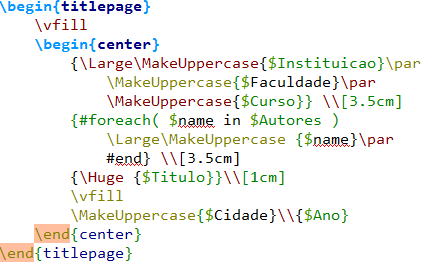
\includegraphics[width=3.07292in,height=1.96875in]{Cap02-img/Cap02-img001.png} 
\fonte{Autoria pr\'opria}} 
\end{figure}

{



\bigskip

\subsection[Writer2Latex]{ Writer2Latex}

\bigskip

{
\textrm{A API open source\ Writer2{\LaTeX} est\'a sendo utilizada no desenvolvimento do TCCTeX, pois reconhece todos
textos, tabelas e figuras que existem em um documento ODT (}\textrm{\textit{open document text}}\textrm{) e a partir
desse reconhecimento converte o arquivo para {\LaTeX}.}}

{
Essa convers\~ao s\'o \'e poss\'ivel\ por meio de um arquivo de configura\c{c}\~ao, onde dever\'a estar escrito como o
documento {\LaTeX} dever\'a se comportar, como por exemplo: n\~ao dever\'a existir par\'agrafos sem texto ou muitos
pulos de linha, cap\'itulos e sub cap\'itulos dever\~ao ser substitu\'idos pelo c\'odigo\ declarado, entre outras
coisas.}


\bigskip

{


\begin{figure}[H]
\caption{Exemplo de Configura\c{c}\~ao Writer2Latex}}
 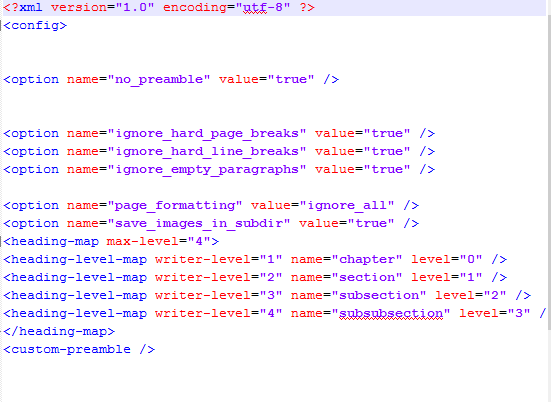
\includegraphics[width=4.8125in,height=3.51042in]{Cap02-img/Cap02-img002.png} 
\fonte{Autoria pr\'opria}} 
\end{figure}

{



\bigskip


\bigskip

{
\textrm{O Writer2Latex consegue fazer o seu papel de converter um arquivo\ }\textrm{\textit{Opendocument}}\textrm{\ para
{\LaTeX} muito bem, mas adiciona ao documento gerado v\'arias linhas de c\'odigo desnecess\'arias para nosso projeto,
al\'em disso n\~ao consegue reconhecer padr\~oes de legendas de figuras e tabelas, nem deixar o documento gerado no
padr\~ao ABNT, mas o TCCTeX conseguir\'a suprir todos estes problemas.}}
null
\chapter{DESENVOLVIMENTO DO PROJETO}

\bigskip


A metodologia de\ \textit{Extreme Programming}\ (XP) foi escolhida, devido ao fato de estar muito relacionada a
agilidade e flexibilidade, caracter\'isticas essas que\ condiziam com a forma como desej\'avamos trabalhar.

Logo em seguida notamos que, antes de iniciar o desenvolvimento do software, dever\'iamos dividir nossa equipe em tr\^es
frentes de trabalho, para que pud\'essemos desenvolver o projeto com mais agilidade e efici\^encia. Elas se
comunicariam com frequ\^encia e trocariam suas experi\^encias pesquisas e conclus\~oes a cada etapa que fosse superada.
As tr\^es frentes de trabalho que eram divididas em A, B e C tinham as seguintes fun\c{c}\~oes:


\bigskip

\liststyleLFOi
\begin{itemize}
\item {
Frente de trabalho A: Verificar quais\ as exig\^encias da Metodista em rela\c{c}\~ao \`a padroniza\c{c}\~ao ABNT e
planejar como nosso software ira auxiliar o usu\'ario a atender essas exig\^encias.}
\item {
\textrm{Frente de trabalho B: Pesquisar como funciona a metodologia escolhida para desenvolver o software e preparar a
equipe do projeto para aplicar essa metodologia.}}
\item {
\textrm{Frente de trabalho C: Pesquisar e aprender como utilizar as tecnologias que iriam permitir o desenvolvimento do
TCCTeX e como seria feita a intera\c{c}\~ao dessas tecnologias.\ }}
\end{itemize}

\bigskip

Essas tr\^es frentes de trabalho foram, como previsto, naturalmente se complementando e conforme as atividades de uma
frente avan\c{c}avam elas alcan\c{c}avam um n\'ivel o qual dependeriam da intera\c{c}\~ao com outra frente de trabalho
para se desenvolver.\ 

A primeira frente de trabalho que alcan\c{c}ou esse n\'ivel foi a frente de trabalho A que conseguiu captar as
necessidades que o software deveria suprir e planejar como ele iria interagir com o usu\'ario desenvolvendo
prot\'otipos visuais do TCCTeX. A partir dessa conclus\~ao a frente de trabalho A passou a trabalhar em\ conjunto com a
frente C para encontrar as tecnologias e ferramentas que viabilizariam o desenvolvimento do software dentro desses
par\^ametros e discutir poss\'iveis altera\c{c}\~oes dos prot\'otipos em prol de melhorias nas funcionalidades do
TCCTeX.

Em seguida a frente de trabalho B conseguiu estabelecer como iriamos aplicar a metodologia XP em nosso projeto e passou
a toda a equipe do projeto como seriam implantada a metodologia e como ela iria auxiliar no desenvolvimento do
software.\ 


A frente de trabalho C, por\ sua vez conseguiu encontrar diversas tecnologias que poderiam possibilitar no
desenvolvimento do software e passou a testa-las para verificar a efici\^encia de cada uma delas e escolher quais
melhor se adequavam com as necessidades do software. A frente de trabalho C s\'o concluiria esse processo de pesquisa e
escolha durante o desenvolvimento do software, pois seria durante o desenvolvimento do software que essas tecnologias e
a capacidade de intera\c{c}\~ao delas seriam realmente posta a prova.


\bigskip

\section{APLICA\c{C}\~AO DA METODOLOGIA XP}

\bigskip

Com base em nossos estudos sobre Extreme Programming (XP) notamos que essa metodologia requer contato direto e
recorrente do cliente do projeto em desenvolvimento e neste quesito notamos uma diferen\c{c}a entre o nosso projeto e
outros projetos desenvolvidos utilizando XP, pois como alunos da Universidade Metodista de S\~ao Paulo, n\'os podemos
assumir o papel tanto de clientes desse projeto como de desenvolvedores do mesmo.


A partir do momento em que come\c{c}amos a aplicar XP na pr\'atica tivemos que nos conscientizar dos dois pap\'eis que
exercemos e como lidar com essa dualidade sem prejudicar o andamento do projeto nem no produto final.


Para suprir a impossibilidade da equipe de nos reunir e compartilhar um espa\c{c}o de trabalho \'unico, portanto, n\~ao
termos um local f\'isico para colocarmos um quadro de tarefas ou de cart\~oes de hist\'oria, utilizamos a ferramenta de
anota\c{c}\~oes Microsoft Office OneNote combinado com o servi\c{c}o de armazenamento e partilha de arquivos Dropbox.
Essa uni\~ao nos possibilitou a flexibilidade do\ planejamento do projeto tal qual \'e previsto na metodologia XP.\ 

Para iniciar o projeto aplicando XP dever\'iamos assumir o papel de clientes e escrever cart\~oes de\ hist\'oria (User
Stories) contando o que um aluno da UMESP que est\'a desenvolvendo a documenta\c{c}\~ao\ do seu TCC deseja que o
software TCCTeX fa\c{c}a por ele. Para escrever as hist\'orias de usu\'ario t\'inhamos o seguinte modelo:


\bigskip




\begin{figure}[H]
\caption{Modelo de User Stories}
 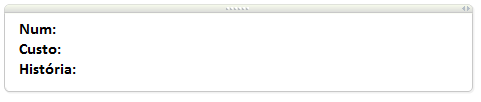
\includegraphics[width=5.01319in,height=1.06528in]{Cap03-img/Cap03-img001.png} 
\fonte{Autoria pr\'opria}} 
\end{figure}





\bigskip

O qual deveria ser usado seguindo a seguinte referencia:

\liststyleLFOii
\begin{itemize}
\item {
\textbf{Num:}\ n\'umero de\ identifica\c{c}\~ao do cart\~ao.}
\item {
\textbf{Custo:\ }estimativa de custo de tempo de 1 \`a 3 semanas que deve ser feita em grupo.}
\item {
\textbf{Hist\'oria:}\ n\'os, no papel de clientes, dever\'iamos escrever hist\'orias de o que gostar\'iamos que o
software fizesse\ evitando termos t\'ecnicos.}
\end{itemize}

\bigskip

Cada uma dessas hist\'orias representa uma parte de software que pode ser entregue a parte.\ Ap\'os escrever as
hist\'orias n\'os em grupo, assumindo o papel de desenvolvedores dever\'iamos fazer uma Reuni\~ao de Planejamento de
Releases (entregas, libera\c{c}\~oes do software) onde estim\'avamos o tempo que levar\'iamos para transformar cada uma
dessas hist\'orias em c\'odigo e em seguida escolh\'iamos quais hist\'orias desenvolver\'iamos primeiro.

Estas hist\'orias eram organizadas, j\'a na ordem de desenvolvimento em um documento do One Note chamado Plano de
Libera\c{c}\~ao que continha tamb\'em os Testes Funcionais que eram desenvolvidos durante as\ Reuni\~oes de
Planejamento de Itera\c{c}\~oes.

Os\ Testes Funcionais representam o resultado esperado do sistema. Cada hist\'oria possui um ou mais Testes Funcionais
que eram\ ser aplicados para verificar se essa hist\'oria foi completamente implementada. Cada um dos Testes Funcionais
possu\'ia uma caixa de sele\c{c}\~ao que tinham a seguinte fun\c{c}\~ao:


\bigskip



\begin{figure}[H]
\caption{Caixa de Sele\c{c}\~ao dos Testes Funcionais}
 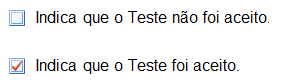
\includegraphics[width=2.97431in,height=0.87014in]{Cap03-img/Cap03-img002.png} 
\fonte{Autoria pr\'opria}} 
\end{figure}

\bigskip


Fizemos Testes Funcionais simples e de f\'acil verifica\c{c}\~ao visual.

Decidimos que far\'iamos itera\c{c}\~oes de uma semana com Reuni\~oes de Planejamento de Itera\c{c}\~ao no inicio de
cada semana. As reuni\~oes tinham como objetivo dividir hist\'orias em tarefas, decidir quais tarefas seriam
desenvolvidas durante a semana e escrever\ Testes Funcionais. Faz\'iamos tamb\'em reuni\~oes ao final de cada semana
que eram utilizadas para verificar os resultados da semana e propor poss\'iveis novas tarefas a partir das
experi\^encias da semana que se passou.

As tarefas que s\~ao planejadas s\~ao escritas seguindo o seguinte modelo:

\bigskip


\begin{figure}[H]
\caption{Modelo de Cart\~ao de Tarefa}
 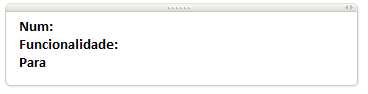
\includegraphics[width=3.83125in,height=0.97431in]{Cap03-img/Cap03-img003.png} 
\fonte{Autoria pr\'opria}} 
\end{figure}

\bigskip

O qual deveria ser usado seguindo a seguinte referencia:

\liststyleLFOii
\begin{itemize}
\item {
\textbf{Num:}\ neste campo ser\'a colocado um numero ser\'a utilizado para\ fazer a referencia entre o cart\~ao de
hist\'oria de usu\'ario e cada tarefa.}
\item {
\textbf{Funcionalidade:}\ aquilo que deve ser desenvolvido.}
\item {
\textbf{Para:\ }motiva\c{c}\~ao pela qual se deseja que essa tarefa seja implementada. \'E utilizado para evitar que o
uma funcionalidade desnecess\'aria\ seja desenvolvida.}
\end{itemize}

\bigskip

Todas as tarefas eram organizadas em um documento do One Note chamado Tarefas do TCCTeX que era dividido em tr\^es
colunas:

\liststyleLFOii
\begin{itemize}
\item {
\textbf{N\~ao Implantadas:\ }tarefas que devem ser desenvolvidas, mas que ainda n\~ao foram designadas para nenhuma
itera\c{c}\~ao;}
\item {
\textbf{Em Itera\c{c}\~ao:\ }tarefas que foram designadas para a pr\'oxima itera\c{c}\~ao;}
\item {
\textbf{Finalizadas:}\ tarefas que j\'a passaram por itera\c{c}\~oes e est\~ao finalizadas.}
\end{itemize}

\bigskip

Durante as Reuni\~oes de Planejamento de Itera\c{c}\~ao, quando decid\'iamos que iriamos desenvolver certa tarefa
durante a pr\'oxima itera\c{c}\~ao n\'os mov\'iamos o cart\~ao desta tarefa para a coluna ``Em Itera\c{c}\~ao'' e em
seguida copi\'avamos essa tarefa para o documento do One Note chamado Plano de Itera\c{c}\~ao.

O Plano de Itera\c{c}\~ao era dividido horizontalmente em semanas/itera\c{c}\~oes e verticalmente\ em tr\^es colunas:

\liststyleLFOii
\begin{itemize}
\item {
\textbf{N\~ao Implantadas:\ }tarefas que devem ser desenvolvidas;}
\item {
\textbf{Em Desenvolvimento:\ }tarefas que est\~ao sendo implementadas por um dos desenvolvedores;}
\item {
\textbf{Finalizadas:}\ tarefas que j\'a tiveram suas funcionalidades desenvolvidas.}
\end{itemize}

\bigskip

\section{ARQUITETURA DO SOFTWARE UTILIZANDO ODT}

\bigskip

O software tem uma arquitetura complexa em decorr\^encia da necessidade do TCCTeX tem suprir a de grande quantidade de
normas exigidas pela para a elabora\c{c}\~ao da documenta\c{c}\~ao do TCC pela Universidade Metodista de S\~ao Paulo.

Abaixo disponibilizamos uma figura que demonstra a arquitetura criada para gerar os arquivos .tex a partir dos arquivos
.odt e algumas informa\c{c}\~oes espec\'ificas.


\bigskip

{


\begin{figure}[H]
\caption{Parte da arquitetura do software TCCTeX}}
 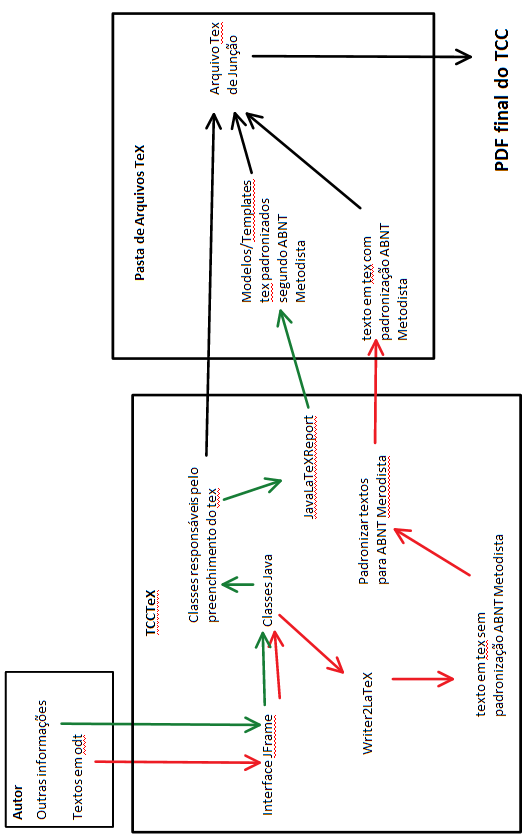
\includegraphics[width=5.49375in,height=8.74028in]{Cap03-img/Cap03-img004.png} 
\fonte{Autoria pr\'opria}} 
\end{figure}

{



\bigskip

\section{FUNCIONAMENTO DO TCCTEX}

\bigskip

{
Neste\ subcap\'itulo explicaremos o funcionamento do software TCCTeX.}

{
O programa se estrutura em 4 pacotes, pacotes de c\'odigos-fonte (padr\~ao do java), pacotes de teste, bibliotecas
(padr\~ao do java), bibliotecas de testes.\ }


\bigskip

{


\begin{figure}[H]
\caption{Projeto \ TCCTeX}}
 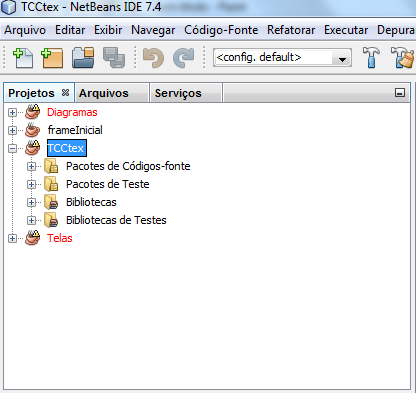
\includegraphics[width=5.22083in,height=4.09097in]{Cap03-img/Cap03-img005.png} 
\fonte{Autoria pr\'opria}} 
\end{figure}

{



\bigskip

{
Pacotes de c\'odigos-fonte s\~ao utilizados para abrigar os pacotes divididos em responsabilidades, no software TCCTeX
temos 3 pacotes principais, br.metodista.TCCtex, br.metodista.TCCtex.telas, br.metodista.TCCTex.telas.imagens.}




{


\begin{figure}[H]
\caption{Pacotes do TCCTeX}}
 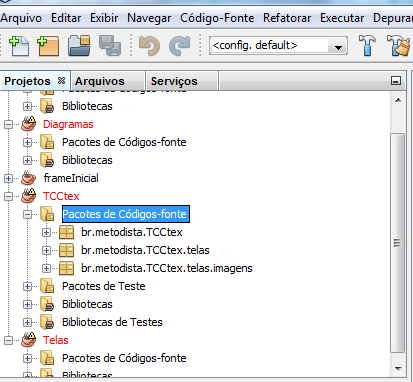
\includegraphics[width=3.94792in,height=3.63611in]{Cap03-img/Cap03-img006.png} 
\fonte{Autoria pr\'opria}} 
\end{figure}




\subsection{Pacote br.metodista.TCCtex}


Este pacote cont\'em as classes java Conversor, Figura, infoEssenciais, PreTextuais, Principal e Textuais.\ 




{


\begin{figure}[H]
\caption{Pacote br.metodista,TCCTeX}
 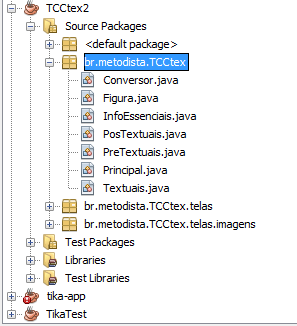
\includegraphics[width=3.09444in,height=3.39653in]{Cap03-img/Cap03-img007.png} 
\fonte{Autoria pr\'opria}} 
\end{figure}

{



\bigskip

\subsubsection{Classe Conversor}

\bigskip

{
Esta classe \'e utilizada para convers\~ao, padroniza\c{c}\~ao e gera\c{c}\~ao de arquivos no formato tex e pdf. Na
classe Conversor, como em todas as outras, se faz necess\'ario a importa\c{c}\~oes de pacotes.}


\bigskip

{


\begin{figure}[H]
\caption{Importa\c{c}\~oes da Classe Conversor}}
 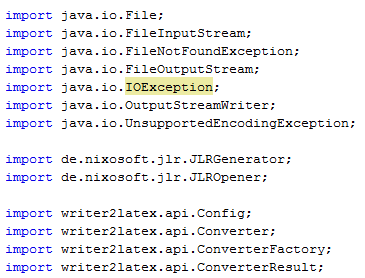
\includegraphics[width=3in,height=2.28333in]{Cap03-img/Cap03-img008.png} 
\fonte{Autoria pr\'opria}} 
\end{figure}

{



\bigskip

{
\textrm{Utilizamos pacotes para organizar as classes, que atuam com um mesmo grupo de caracter\'isticas, o pacote
de.nixosoft.jlr.JLRGenerator por exemplo \'e utilizado no preenchimento de templates feitos em {\LaTeX}, como citado
anteriormente, j\'a o pacote nixosoft.jlr.JLROpener \'e utilizado para convers\~ao de documentos {\LaTeX} para PDF e
possui um m\'etodo open(File) para abrir mais rapidamente o PDF gerado.}}


\bigskip

{


\begin{figure}[H]
\caption{JLR para Gera\c{c}\~ao de PDF}}
 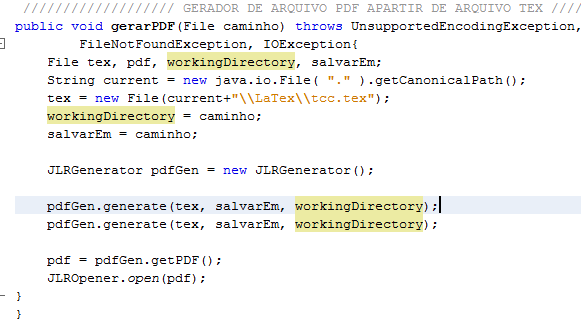
\includegraphics[width=4.34306in,height=2.43264in]{Cap03-img/Cap03-img009.png} 
\fonte{Autoria pr\'opria}} 
\end{figure}

{



\bigskip

{
O pacote writer2latex.api possui a classe\ \textit{Config\ }que armazena o local do arquivo xml de configura\c{c}\~ao do
writer2{\LaTeX} e algumas de suas configura\c{c}\~oes podem ser escritas diretamente na classe java como no exemplo
abaixo onde config.setOption(``inpuntencoding'',''UTF-8'') significa que os arquivos ODT devem ser abertos utilizando o
padr\~ao de codifica\c{c}\~ao UTF-8.}


\bigskip

{


\begin{figure}[H]
\caption{M\'etodo odtToTex}}
 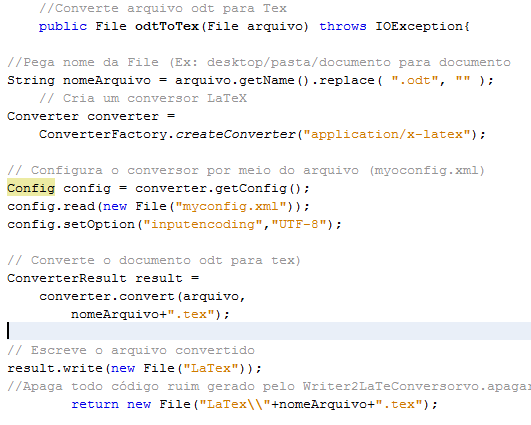
\includegraphics[width=3.88333in,height=3.10417in]{Cap03-img/Cap03-img010.png} 
\fonte{Autoria pr\'opria}} 
\end{figure}

{



\bigskip

{
A classe\ \textit{Converter}\ \'e utilizada para convers\~ao do arquivo ODT para um texto no padr\~ao {\LaTeX}, \ j\'a a
classe CoverterResult recebe esse texto e o escreve em um\ arquivo com a extens\~ao tex.}


\bigskip

{


\begin{figure}[H]
\caption{Parte do M\'etodo alterarTex()}}
 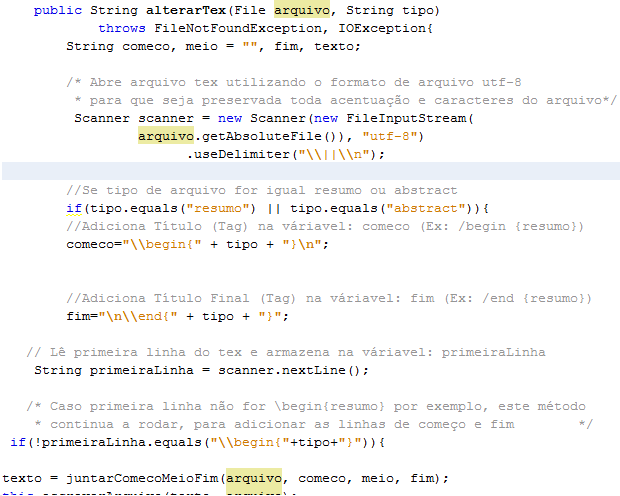
\includegraphics[width=4.62361in,height=3.68819in]{Cap03-img/Cap03-img011.png} 
\fonte{Autoria pr\'opria}} 
\end{figure}

{



\bigskip

{
Seguindo na classe Conversor, temos um outro m\'etodo, chamado alterarTex(), que possui algumas fun\c{c}\~oes como ler o
arquivo convertido pelo Writer2{\LaTeX}, verificar\ se o arquivo \'e o resumo, abstract, dedicat\'oria, etc, adicionar
o t\'itulo se necess\'ario conforme o tipo de arquivo e utilizar outros m\'etodos para remover c\'odigo desnecess\'ario
gerado pelo Writer2{\LaTeX} e reescrever o arquivo tex.}


\bigskip

\subsubsection{Classe InfoEssenciais}

\bigskip

{
A classe InfoEssenciais recebe v\'arias informa\c{c}\~oes necess\'arias para gera\c{c}\~ao da capa, folha de rosto e
folha de aprova\c{c}\~ao, al\'em de gerar uma ficha catalogr\'afica n\~ao preenchida para que pr\'evias do TCC possam
ser entregues, no pr\'oximo exemplo \'e demonstrado um m\'etodo utilizado para gera\c{c}\~ao desses arquivos.}


\bigskip

{


\begin{figure}[H]
\caption{JLR para Preenchimento de Template Tex}}
 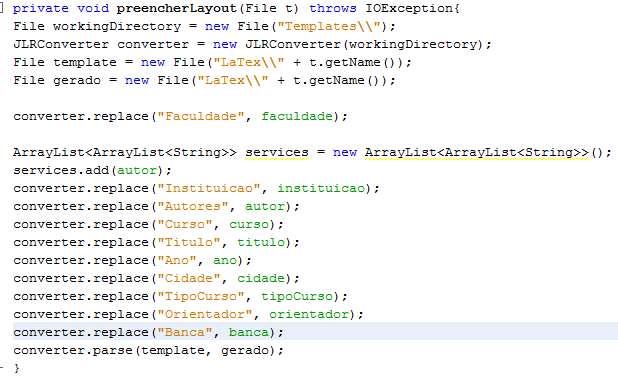
\includegraphics[width=4.85694in,height=2.94792in]{Cap03-img/Cap03-img012.png} 
\fonte{Autoria pr\'opria}} 
\end{figure}

{



\bigskip

\subsubsection{Classe PreTextuais}

\bigskip

{
A classe PreTextuais recebe os arquivos Odt contendo o resumo, abstract, dedicat\'oria, agradecimentos e epigrafe e faz
a convers\~ao dos mesmos para tex se os arquivos obrigat\'orios resumo e abstract existirem.}


\bigskip

{


\begin{figure}[H]
\caption{M\'etodo converterPre()}}
 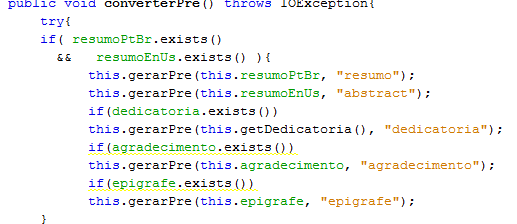
\includegraphics[width=5.38958in,height=2.3375in]{Cap03-img/Cap03-img013.png} 
\fonte{Autoria pr\'opria}} 
\end{figure}

{



\bigskip


\bigskip


\bigskip


\bigskip


\bigskip


\bigskip

\subsubsection{Classe Textuais}

\bigskip

{
A classe Textuais possui algumas vari\'aveis que guardam o caminho de cada arquivo\ utilizado na etapa de Textuais,
s\~ao estas as vari\'aveis introdu\c{c}\~ao e conclus\~ao do tipo\ \textit{File}\ e a lista de cap\'itulos tamb\'em do
tipo\ \textit{File}.}


\bigskip

{


\begin{figure}[H]
\caption{Classe textuais}}
 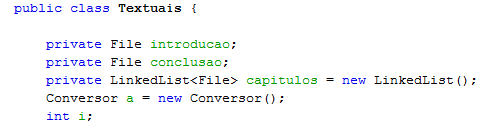
\includegraphics[width=5.14931in,height=1.37292in]{Cap03-img/Cap03-img014.png} 
\fonte{Autoria pr\'opria}} 
\end{figure}

{



\bigskip

{
O m\'etodo listarImagens() da classe Textuais reconhece todas\ legendas de figuras criadas no software Microsoft Word e
coloca no padr\~ao {\LaTeX} corretamente para que possa ser gerada a numera\c{c}\~ao de cada figura e a lista contendo
todas. No pequeno trecho retirado do m\'etodo listarImagens(), mostrado na pr\'oxima figura, \'e\ demonstrado como as
legendas s\~ao reconhecidas pelo software para que posteriormente sejam tratadas e gerado o c\'odigo correto das
mesmas.}


\bigskip


\bigskip

{


\begin{figure}[H]
\caption{M\'etodo converterTextuais()}}
 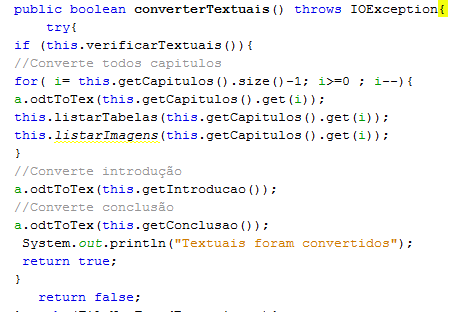
\includegraphics[width=4.31181in,height=2.92222in]{Cap03-img/Cap03-img015.png} 
\fonte{Autoria pr\'opria}} 
\end{figure}

{



\bigskip

\subsubsection{Classe Principal}

\bigskip

{


\begin{figure}[H]
\caption{Parte do m\'etodo abrir() Principal}}
 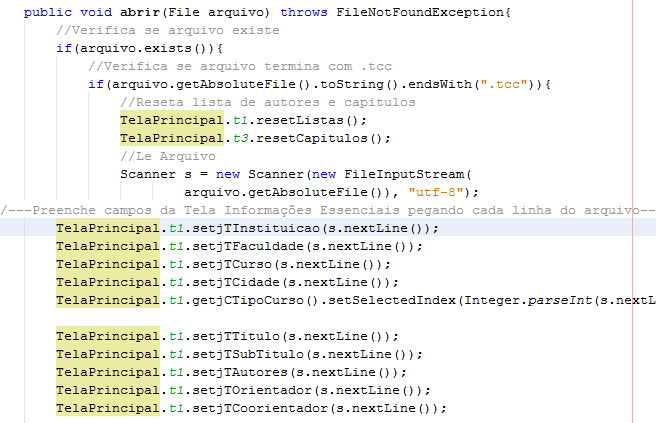
\includegraphics[width=5.90556in,height=3.80934in]{Cap03-img/Cap03-img016.png} 
\fonte{Autoria pr\'opria}} 
\end{figure}

{



\bigskip

{
A Classe principal tem a fun\c{c}\~ao de gerar o arquivo que salva o projeto desenvolvido pelo usu\'ario e de carregar
esse mesmo arquivo, assim o usu\'ario pode salvar o um projeto em andamento e continuar mais tarde.}


\bigskip

\subsection[Pacote\ br.metodista.TCCtex.telas]{Pacote\ br.metodista.TCCtex.telas}

\bigskip

{


\begin{figure}[H]
\caption{Pacote Contendo as Telas}}
 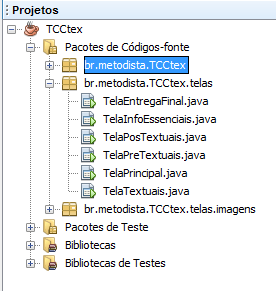
\includegraphics[width=2.36389in,height=2.49375in]{Cap03-img/Cap03-img017.png} 
\fonte{Autoria pr\'opria}} 
\end{figure}

{



\bigskip

{
O pacote br.metodista.TCCtex.telas, possui os formul\'arios da aplica\c{c}\~ao, esses formul\'arios s\~ao JFrames, que
nada mais \'e que uma classe, especializada em componentes visuais, como bot\~oes, menus, caixas de texto, e tudo que
existem em janelas de aplicativos.}


\bigskip

\subsubsection{Pacote br.metodista.TCCTex.telas.imagens}

\bigskip

{


\begin{figure}[H]
\caption{Pacote Contendo Imagens}}
 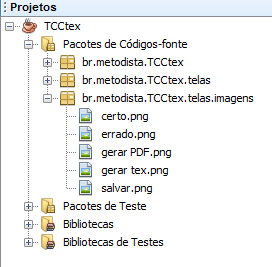
\includegraphics[width=2.22083in,height=2.18194in]{Cap03-img/Cap03-img018.png} 
\fonte{Autoria pr\'opria}} 
\end{figure}

{



\bigskip

{
As boas pr\'aticas da linguagem java, tanto em aplica\c{c}\~oes desktop, quanto WEB, sugerem que os arquivos de imagens
fiquem em um pacote dedicado, na nossa aplica\c{c}\~ao esse pacote \'e o br.metodista.TCCtex.telas.imagens, dentro dele
temos as imagens usadas no aplicativo.}


\bigskip

\section{INTERFACES}

\bigskip

{
O design e funcionamento das interfaces foram feitos de forma a garantir o processo de aprendizagem e uso o mais simples
poss\'ivel, para o usu\'ario final.\ }


\bigskip

\subsection{INTERFACE DA TELA PRINCIPAL}

\bigskip

{
A tela principal \'e composta por: bot\~oes de cada etapa a ser realizada para que o trabalho possa ser
finalizado,\ sendo indicado se determinada etapa foi conclu\'ida ou n\~ao ao seu lado por uma imagem; bot\~ao Salvar,
para guardar todas as informa\c{c}\~oes preenchidas pelo usu\'ario em todas as interfaces gr\'aficas; bot\~ao Gerar PDF
para converter o trabalho gerado de {\LaTeX} para PDF, salvando-o no local onde o usu\'ario desejar.}


\bigskip

{


\begin{figure}[H]
\caption{Interface da Tela Principal}}
 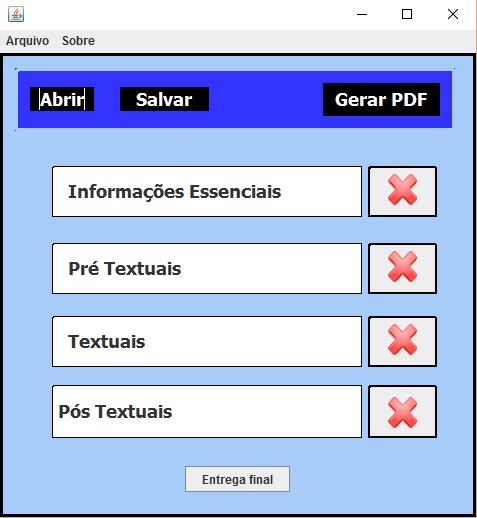
\includegraphics[width=4.97014in,height=5.40278in]{Cap03-img/Cap03-img019.png} 
\fonte{Autoria pr\'opria}} 
\end{figure}

{



\bigskip

{
Quando o usu\'ario conclui determinada etapa a imagem ao lado da op\c{c}\~ao da etapa \'e alterada para indicar que a
mesma foi conclu\'ida.}


\bigskip

{


\begin{figure}[H]
\caption{Etapa Conclu\'ida}}
 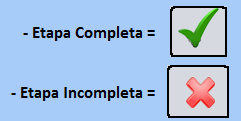
\includegraphics[width=2.50625in,height=1.25972in]{Cap03-img/Cap03-img020.png} 
\fonte{Autoria pr\'opria}} 
\end{figure}

{



\bigskip

\subsection{INTERFACE DA TELA DE INFORMA\c{C}\~OES ESSENCIAIS}

\bigskip

{
A tela de informa\c{c}\~oes essenciais possui os campos de texto: nome da institui\c{c}\~ao, faculdade, curso, cidade da
institui\c{c}\~ao, t\'itulo do trabalho, subt\'itulo, autores, orientador, coorientador(es) e ano de entrega. Tamb\'em
possui o bot\~ao voltar e as caixas de sele\c{c}\~ao: tipo de curso, natureza e terminei esta parte que ao ser clicada
verifica se o usu\'ario preencheu todas informa\c{c}\~oes necess\'arias, caso ele tenha preenchido, s\~ao gerados
arquivos {\LaTeX} para a capa, ficha catalogr\'afica, folha de aprova\c{c}\~ao e folha de rosto, retornando o usu\'ario
para a tela inicial.\ }


\bigskip

{


\begin{figure}[H]
\caption{Interface da Tela de Informa\c{c}\~oes Essenciais}}
 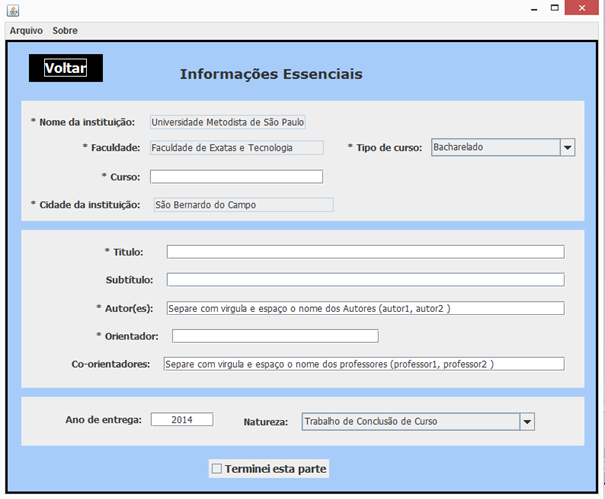
\includegraphics[width=5.83125in,height=4.80486in]{Cap03-img/Cap03-img021.png} 
\fonte{Autoria pr\'opria}} 
\end{figure}

{



\bigskip

\subsection{INTERFACE DA TELA DE PR\'E-TEXTUAIS}

\bigskip


\bigskip

{
Na tela de pr\'e-textuais o usu\'ario dever\'a inserir arquivos com o resumo do trabalho em portugu\^es e ingl\^es
(\textit{abstract}), poder\'a tamb\'em inserir arquivos de texto como a errata, dedicat\'oria, agradecimentos e
epigrafe, sendo que n\~ao dever\'a escrever o t\'itulo de cada parte do trabalho nos documentos. O usu\'ario poder\'a
abrir os documentos ap\'os seleciona-los para efetuar modifica\c{c}\~oes clicando no bot\~ao: abrir. A caixa de
sele\c{c}\~ao: Terminei esta parte ir\'a verificar se o usu\'ario inseriu todos arquivos obrigat\'orios, assim os
convertendo para {\LaTeX} no padr\~ao ABNT utilizado pela metodista.}


\bigskip

{


\begin{figure}[H]
\caption{Interface da tela de Pr\'e-Textuais}}
 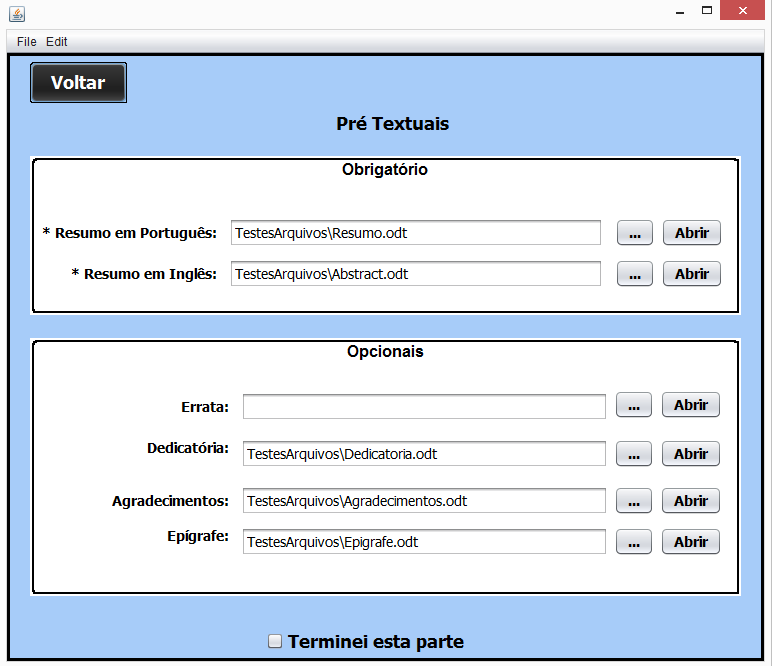
\includegraphics[width=5.73125in,height=4.92569in]{Cap03-img/Cap03-img022.png} 
\fonte{Autoria pr\'opria}} 
\end{figure}

{



\bigskip

\subsection{INTEFACE DA TELA DE TEXTUAIS}

\bigskip

{
Nesta tela o usu\'ario dever\'a inserir arquivos ODT contendo: a introdu\c{c}\~ao, todos cap\'itulos\ separados e
conclus\~ao, o arquivo onde estar\'a escrito cada um, podendo conter tabelas e imagens, tamb\'em poder\'a adicionar
novos cap\'itulos, remove-los e abrir o arquivo para edi\c{c}\~ao.\ }

{
Ao clicar na op\c{c}\~ao: terminei esta parte os arquivos inseridos ser\~ao convertidos para {\LaTeX}, no padr\~ao ABNT
da Metodista.}

{


\begin{figure}[H]
\caption{Interface da Tela de Textuais}}
 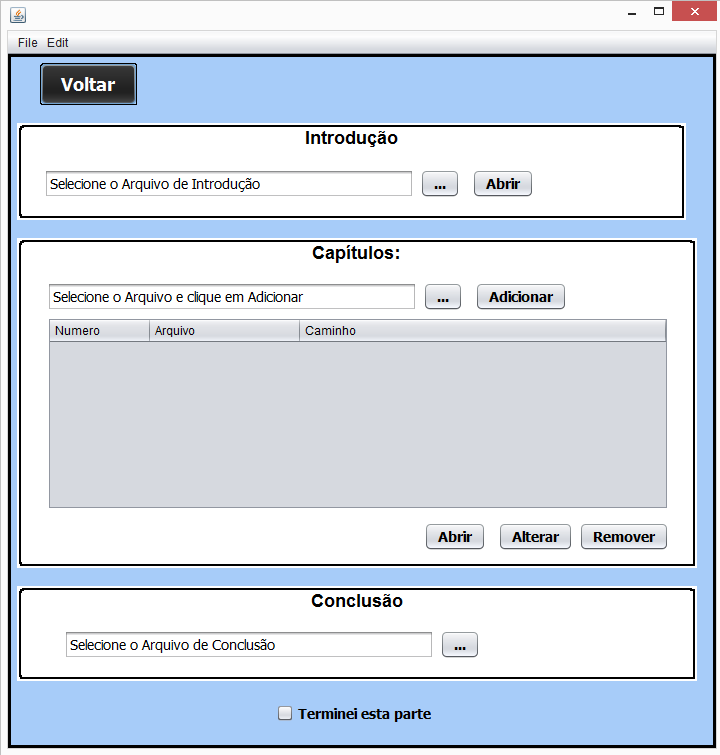
\includegraphics[width=5.75347in,height=6.03889in]{Cap03-img/Cap03-img023.png} 
\fonte{Autoria pr\'opria}} 
\end{figure}

{



\bigskip

\subsection{INTERFACE DA TELA P\'OS-TEXTUAIS}

\bigskip

{
Por meio desta tela ser\'a poss\'ivel inserir um arquivo com todas refer\^encias citadas no texto, para isso o usu\'ario
poder\'a utilizar o sistema Online MORE para criar as cita\c{c}\~oes e refer\^encias e colar as mesmas no documento a
ser inserido. Alguns anexos s\~ao obrigat\'orios, sendo o Relat\'orio de recomenda\c{c}\~oes da banca de
qualifica\c{c}\~ao (RRBQ) um deles. O anexo contendo todas\ Atas e Cronogramas desenvolvidos durante o curso devem ser
estregues no desenvolvimento da entrega final do TCC, sendo assim podem ser adicionados ao documento, caso o usu\'ario
n\~ao esteja fazendo uma pr\'evia do trabalho.}


\bigskip

{


\begin{figure}[H]
\caption{Interface da Tela P\'os-Textuais}}
 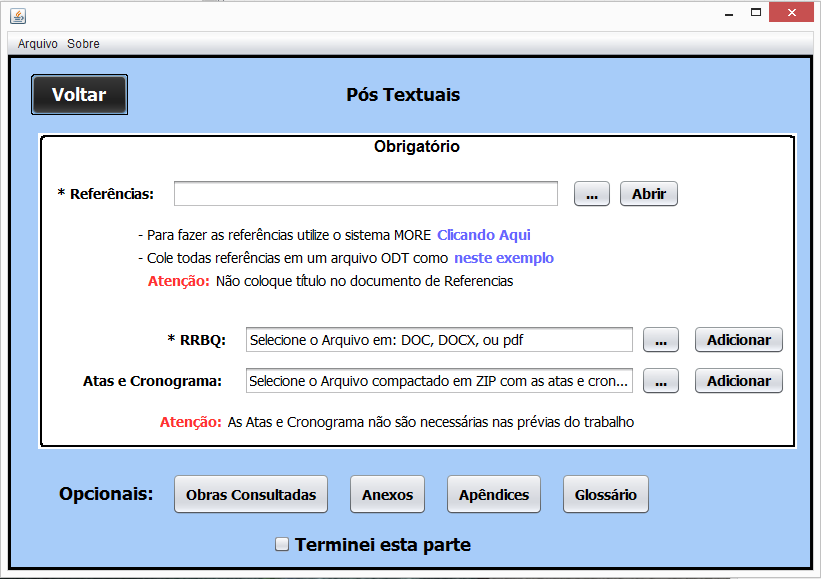
\includegraphics[width=5.89583in,height=4.14931in]{Cap03-img/Cap03-img024.png} 
\fonte{Autoria pr\'opria}} 
\end{figure}

{



\bigskip

\subsection{INTERFACE DA TELA ENTREGA FINAL}

\bigskip

{
A tela de entrega final \'e utilizada apenas como o pr\'oprio nome indica, no desenvolvimento do TCC para entrega final,
para isso o aluno ou seu grupo deve procurar auxilio na biblioteca da Universidade Metodista para produ\c{c}\~ao da
ficha catalogr\'afica, ao enviar algumas informa\c{c}\~oes para a biblioteca como: t\'itulo do trabalho, autores,
orientador, assunto, etc, o aluno receber\'a um documento no qual existir\'a informa\c{c}\~oes como a
classifica\c{c}\~ao de assunto e nota\c{c}\~ao do autor para que o mesmo insira nesta tela e seja gerado o trabalho
para impress\~ao.}


\bigskip

{


\begin{figure}[H]
\caption{Interface da Tela Entrega Final}}
 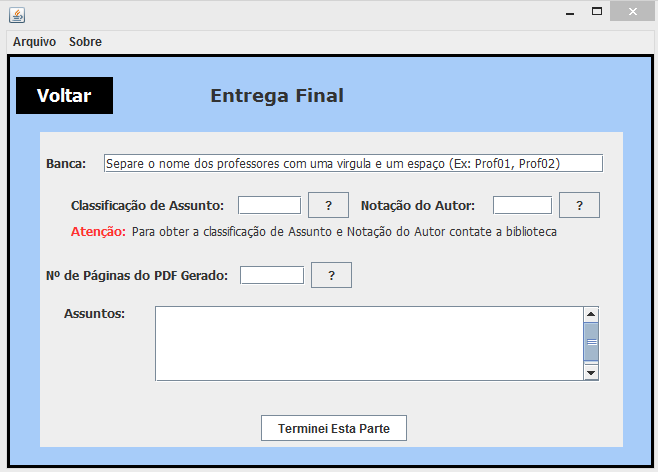
\includegraphics[width=5.90556in,height=4.2354in]{Cap03-img/Cap03-img025.png} 
\fonte{Autoria pr\'opria}} 
\end{figure}

{



\bigskip

\section{REGRAS DE NEG\'OCIO}

\bigskip

{
Aqui estar\~ao listadas algumas regras para que o aluno fa\c{c}a o\ preenchimento da interface:}


\bigskip

{


\begin{center}
\begin{table}
\caption{Regra de Neg\'ocio: Tela Informa\c{c}\~oes Essenciais}}
\tablefirsthead{}

\tablehead{}
\tabletail{}
\tablelasttail{}
\begin{supertabular}{m{1.6837599in}|m{4.04556in}}
\hline
{ Regra de neg\'ocios} &
{ 1}\\\hline
{ Descri\c{c}\~ao}

~

~
 &
{ O aluno deve escrever algumas informa\c{c}\~oes essenciais. Como, nome institui\c{c}\~ao,
faculdade, curso, autores, entres outras.\ }\\\hline
{ Justificativa} &
{ Ao preencher as informa\c{c}\~oes essenciais, \'e gerado um arquivo {\LaTeX} para capa, ficha
catalogr\'afica, folha de aprova\c{c}\~ao e folha de rosto. Caso fosse para inserir arquivos, seria necess\'ario
entradas e telas para cada uma dessas p\'aginas, o que aumentaria o trabalho do aluno}\\\hline
\end{supertabular}
\end{table}
\end{center}
{



\bigskip

{


\begin{center}
\begin{table}
\caption{Regra de Neg\'ocio: Tela Informa\c{c}\~oes Essenciais}}
\tablefirsthead{}

\tablehead{}
\tabletail{}
\tablelasttail{}
\begin{supertabular}{m{1.7003598in}|m{4.06216in}}
\hline
{ Regra de Neg\'ocio} &
{ 2}\\\hline
{ Descri\c{c}\~ao} &
{ Campos em asterisco s\~ao obrigat\'orios.}\\\hline
{ Justificativa} &
{ Informa\c{c}\~oes necess\'arias para os arquivos.}\\\hline
\end{supertabular}
\end{table}
\end{center}
{



\bigskip

{


\begin{center}
\begin{table}
\caption{Regra de Neg\'ocio: Bot\~ao Terminei Esta Parte}}
\tablefirsthead{}

\tablehead{}
\tabletail{}
\tablelasttail{}
\begin{supertabular}{m{1.7191598in}|m{4.0559597in}m{-0.054440156in}}
\hhline{--~}
{ Regra de Neg\'ocio} &
{ 3} &
~
\\\hline
{ Descri\c{c}\~ao} &
\multicolumn{2}{m{4.08026in}}{{ Clicar em terminei esta parte.}}\\\hline
{ Justificativa} &
\multicolumn{2}{m{4.08026in}}{{ Ao clicar nesta marca\c{c}\~ao os arquivos Tex ser\~ao gerados,
e o programa volta para a tela inicial.}}\\\hline
\end{supertabular}
\end{table}
\end{center}
{



\bigskip

{


\begin{center}
\begin{table}
\caption{Regra de Neg\'ocio: Arquivos de Entrada}}
\tablefirsthead{}

\tablehead{}
\tabletail{}
\tablelasttail{}
\begin{supertabular}{m{1.6850599in}|m{4.04626in}}
\hline
{ Regra de Neg\'ocio} &
{ 4}\\\hline
{ Descri\c{c}\~ao\ } &
{ Os arquivos de entradas para transforma\c{c}\~ao no padr\~ao ABNT precisam estar no formato
ODT (Open Document Text) Documento de Texto Aberto.}\\\hline
{ Justificativa} &
{ Por ser Open Source, \'e poss\'ivel\ utilizar junto a v\'arias API's, entre elas o
Writer2Latex a qual estamos usando.}\\\hline
\end{supertabular}
\end{table}
\end{center}
{



\bigskip

{


\begin{center}
\begin{table}
\caption{Regra de Neg\'ocio: Arquivos Opcionais}}
\tablefirsthead{}

\tablehead{}
\tabletail{}
\tablelasttail{}
\begin{supertabular}{m{1.7038599in}|m{4.06496in}}
\hline
{ Regra de Neg\'ocio} &
{ 5}\\\hline
{ Descri\c{c}\~ao} &
{ Arquivos opcionais.}\\\hline
{ Justificativa} &
{ Nem todas as partes de um TCC s\~ao\ obrigat\'orias, algumas s\~ao opcionais como, Errata,
Dedicat\'oria, Ep\'igrafe.}\\\hline
\end{supertabular}
\end{table}
\end{center}
{



\bigskip

{


\begin{center}
\begin{table}
\caption{Regra de Neg\'ocio: Bot\~ao Gerar Tex}}
\tablefirsthead{}

\tablehead{}
\tabletail{}
\tablelasttail{}
\begin{supertabular}{m{1.6934599in}|m{4.0545597in}}
\hline
{ Regra de Neg\'ocio} &
{ 6}\\\hline
{ Descri\c{c}\~ao} &
{ Bot\~ao Gerar Tex funciona apenas se usu\'ario terminou as 4 etapas:
pr\'e-textuais,\ textuais, p\'os-textuais.}\\\hline
{ Justificativa} &
{ Gera os arquivos no formato Tex que poder\'a gerar um arquivo no formato PDF}\\\hline
\end{supertabular}
\end{table}
\end{center}
{



\bigskip

{


\begin{center}
\begin{table}
\caption{Regra de Neg\'ocio: Bot\~ao Gerar PDF}}
\tablefirsthead{}

\tablehead{}
\tabletail{}
\tablelasttail{}
\begin{supertabular}{m{1.7205598in}|m{0.22395986in}m{3.7795599in}}
\hhline{--~}
{ Regra de Neg\'ocio} &
{ 7} &
~
\\\hline
{ Descri\c{c}\~ao} &
\multicolumn{2}{m{4.0822597in}}{{ Bot\~ao Gerar \ PDF funciona se tex foi\ gerado.}}\\\hline
{ Justificativa} &
\multicolumn{2}{m{4.0822597in}}{{ Gera o arquivo no formato pdf. Todas as partes fundamentais
do TCC precisam estar prontas para ser gerado o arquivo.}}\\\hline
\end{supertabular}
\end{table}
\end{center}
{



\bigskip

{


\begin{center}
\begin{table}
\caption{Regra de Neg\'ocio: Adicionar Cap\'itulos da Tela Textuais}}
\tablefirsthead{}

\tablehead{}
\tabletail{}
\tablelasttail{}
\begin{supertabular}{m{1.7177598in}|m{4.07956in}}
\hline
{ Regra de Neg\'ocio} &
{ 8}\\\hline
{ Descri\c{c}\~ao} &
{ Adicionar cap\'itulos}\\\hline
{ Justificativa} &
{ Para que o usu\'ario possa escrever seu arquivo de maneira que achar melhor, n\~ao
necessitando de uma ordem para utilizar o programa.}\\\hline
\end{supertabular}
\end{table}
\end{center}
{



\bigskip

\section{ALTERA\c{C}\~AO DE abnTeX PARA abnTeX2}

\bigskip

{
Para diferenciar a\ vers\~ao original abnTeX do abnTeX2 vamos chamar a vers\~ao original de abnTeX1.}

{
Como o abnTeX1 n\~ao estava catalogada na principal base de dados do {\LaTeX} para utiliza-lo era necess\'ario fazer a
instala\c{c}\~ao manualmente, ainda sim a ultima vers\~ao dispon\'ivel estava\ defasada devido a muitos anos sem
atualiza\c{c}\~oes. Devido a essa defasagem tivemos que adicionar diversos pacotes no arquivo principal do {\LaTeX},
sendo que alguns destes tamb\'em tiveram de ser instalados manualmente para que o pdf final gerado estivesse dentro\ do
padr\~ao ABNT atual. Todo este processo de instala\c{c}\~ao manual de pacotes {\LaTeX} traria grande dificuldade aos
usu\'arios do TCCTeX que nunca haviam utilizado o {\LaTeX} e at\'e mesmo os mais habituados ao {\LaTeX} teriam
dificuldades.}

{
\textrm{Com a altera\c{c}\~ao para o abnTeX2\ estes pacotes n\~ao s\~ao mais necess\'arios pois todos os pacotes
necess\'arios para a formata\c{c}\~ao do documento, bem como o abnTeX2, est\~ao dispon\'iveis do CTAN (Comprehensive
TEX Archive Network) que \'e uma base de dados que possui todo tipo de materiais referentes\ a TeX.\ {}``As principais
distribui\c{c}\~oes LATEX\ s\~ao constru\'idas \`a partir de pacotes e classes do CTAN'' (ARAUJO,2015).}}

{
Com a utiliza\c{c}\~ao do ABNTeX1 houve uma dificuldade maior de aprendizado, pois no site do mesmo n\~ao haviam mais
manuais atualizados de como utiliza-lo e modifica-lo, sendo que tivemos que corrigir diversos problemas do mesmo
reescrevendo diversos comandos.}

{
Com a altera\c{c}\~ao, o c\'odigo fonte do TCCTeX foi alterado em diversos aspectos, removendo coisas desnecess\'arias e
atualizando alguns m\'etodos, como por exemplo m\'etodos relacionados a identifica\c{c}\~ao de figuras, tabelas e o que
deve gerar o arquivo principal com a extens\~ao .tex que conecta todos os outros arquivos tex que formam o documento
PDF do trabalho no padr\~ao ABNT.}

{
Um bom exemplo das modifica\c{c}\~oes que foram feitas no c\'odigo do programa para que ele funcione com abnTeX2 s\~ao
as modifica\c{c}\~oes feitas para a capa e folha de rosto. Como o abnTeX1 estava defasado em rela\c{c}\~ao as ultimas
vers\~oes das normas ABNT era necess\'ario criar templates espec\'ificos para a\ capa e folha de rosto colocando-as na
vers\~ao mais recente das normas ABNT.}

{
Abaixo voc\^e pode verificar uma figura qual era o resultado do preenchimento do template da capa, que gerava o arquivo
``capa.tex'':}


\bigskip

{


\begin{figure}[H]
\caption{Capa em abnTeX1}}
 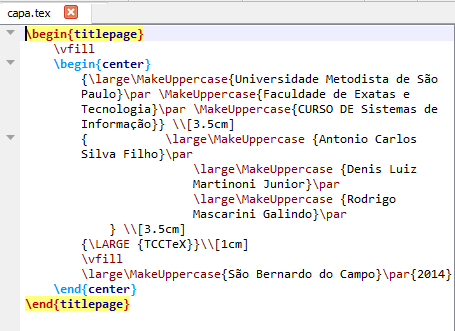
\includegraphics[width=4.74444in,height=3.45347in]{Cap03-img/Cap03-img026.png} 
\fonte{Autoria pr\'opria}} 
\end{figure}

{



\bigskip

{
Abaixo voc\^e pode verificar uma figura qual era o resultado do preenchimento do template da folha de rosto, que gerava
o arquivo ``folharosto.tex'':}


\bigskip

{


\begin{figure}[H]
\caption{Folha de Rosto em abnTeX1}}
 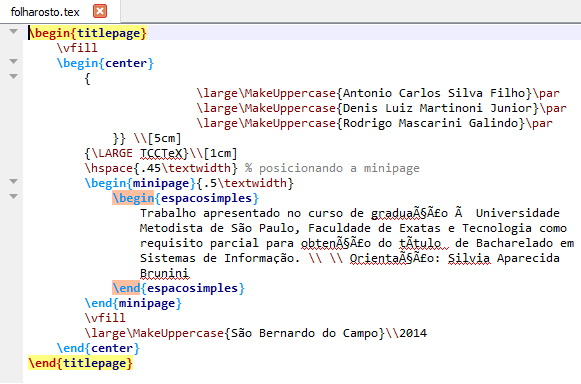
\includegraphics[width=5.89514in,height=3.89514in]{Cap03-img/Cap03-img027.png} 
\fonte{Autoria pr\'opria}} 
\end{figure}

{



\bigskip

{
Quando utilizamos o abnTeX2 s\'o precisamos\ fazer o programa preencher uma s\'erie de macros de dados do documento no
arquivo principal.tex que \'e utilizado para unir todos os arquivos do documento. A figura abaixo mostra como s\~ao
preenchidos esse macros no arquivo principal.tex:}


\bigskip

{


\begin{figure}[H]
\caption{Preenchimento de Macros em principal.tex abnTeX2}}
 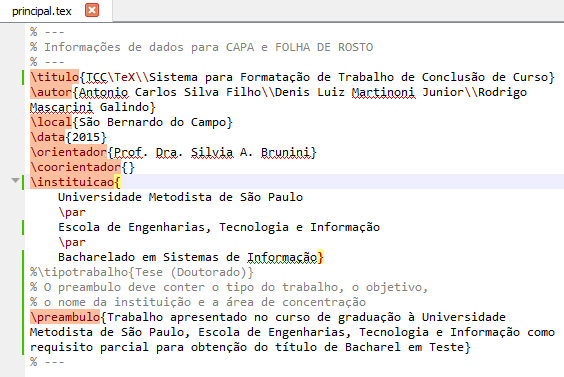
\includegraphics[width=5.88056in,height=3.92569in]{Cap03-img/Cap03-img028.png} 
\fonte{Autoria pr\'opria}} 
\end{figure}

{



\bigskip

{
Ap\'os preencher todos os macros basta utilizar os comandos {\textbackslash}imprimircapa para gerar a capa e
{\textbackslash}imprimirfolhaderosto para gerar a folha de rosto. Esses comandos s\~ao inseridos no pr\'oprio arquivo
principal.tex.}


\bigskip

\section[EXTEN\c{C}\~AO DO PRESENTE TRABALHO]{\textrm{EXTEN\c{C}\~AO DO PRESENTE TRABALHO}}

\bigskip

{
Ap\'os terminar essa fase de desenvolver o software para que ele transforme arquivos em odt para {\LaTeX} colocando-os
dentro dos padr\~oes ABNT, pretendemos desenvolver a mesma funcionalidade para\ transformar arquivos docx em {\LaTeX}
como uma extens\~ao deste projeto.}

{
Para fazer a transforma\c{c}\~ao de textos .docx para um arquivo .tex necessitamos reconhecer os padr\~oes do c\'odigo
xml utilizado pelo docx e comparar com a linguagem {\LaTeX}. Para isso escrevemos\ no Microsoft Word arquivos em docx
com possuem diferentes formata\c{c}\~oes de texto, tabela, imagem e divis\~ao de cap\'itulos, tudo fora da
formata\c{c}\~ao da norma ABNT.\ }


\bigskip

{


\begin{figure}[H]
\caption{Pequeno Texto feito no Microsoft Word}}
 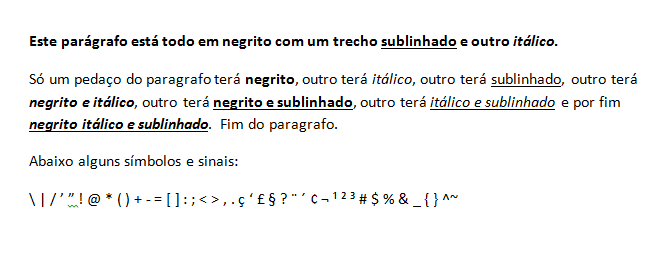
\includegraphics[width=5.90556in,height=2.23174in]{Cap03-img/Cap03-img029.png} 
\fonte{Autoria pr\'opria}} 
\end{figure}

{



\bigskip

{
Em seguida escrevemos, com linguagem {\LaTeX} e utilizando o pacote abnTeX2, arquivos .tex com o mesmo conte\'udo dos
arquivos .docx, por\'em obedecendo as normas abnt.}


\bigskip

{


\begin{figure}[H]
\caption{Pequeno texto em {\LaTeX} com mesmo conte\'udo da figura anterior}}
 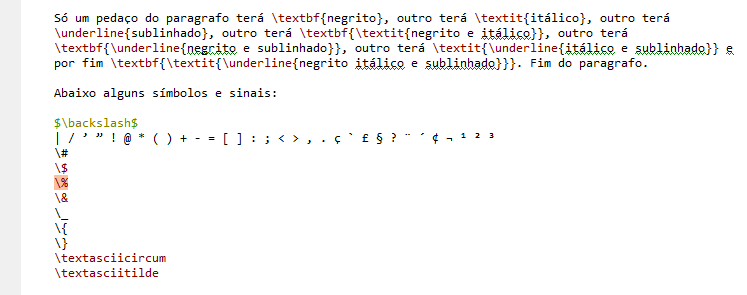
\includegraphics[width=5.90556in,height=2.33366in]{Cap03-img/Cap03-img030.png} 
\fonte{Autoria pr\'opria}} 
\end{figure}

{



\bigskip

{
Em seguida fazemos uma c\'opia do arquivo docx e renomeamos a extens\~ao dessa c\'opia para .zip para assim podermos
descompactar os arquivos xml do docx.}

{
Ap\'os descompactar os arquivos .docx, abrimos, utilizando o NetBeans IDE, o arquivo document.xml que possui o parte
principal do c\'odigo xml\ }


\bigskip

{


\begin{figure}[H]
\caption{Pequena parte do c\'odigo XML do docx}}
 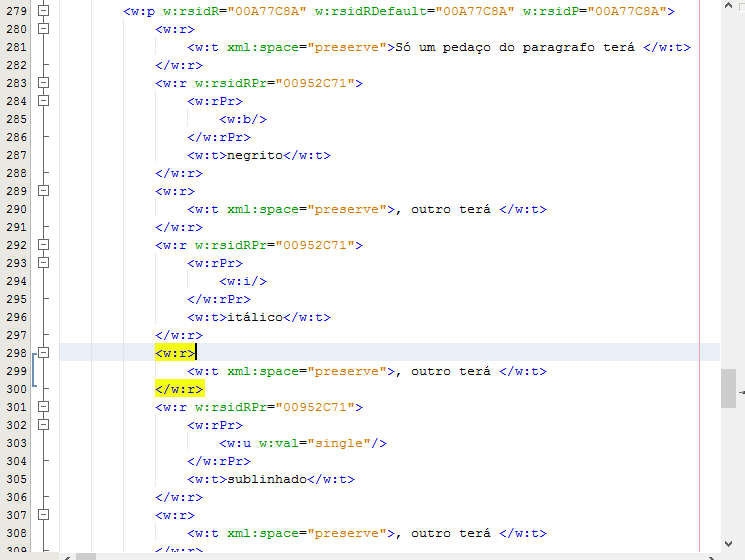
\includegraphics[width=5.90556in,height=4.43403in]{Cap03-img/Cap03-img031.png} 
\fonte{Autoria pr\'opria}} 
\end{figure}

{



\bigskip

{
Este arquivo document.xml \'e bastante extenso e possui todo o conte\'udo inserido no arquivo docx. Cada arquivo docx
possui seu pr\'oprio arquivo document.xml.}

{
\textrm{A partir\ disso teremos que, utilizando o NetBeans IDE, reconhecer os padr\~oes da linguagem xml utilizada no
arquivo .docx, compar\'a-los com os padr\~oes da liguagem {\LaTeX} utilizada no arquivo .tex e criar est\'orias de como
o c\'odigo Java ir\'a converter os arquivos de uma\ linguagem para outra. A partir dessas est\'orias ser\'a criado o
conversor de .docx para {\LaTeX} em Java.\ }}
\include{Conclusao}

\include{Referencias}

%Apendices - Não Implementado
\anexos

\chapter{Relat\'orio de Recomenda\c{c}\~oes da Banca de Qualifica\c{c}\~ao}

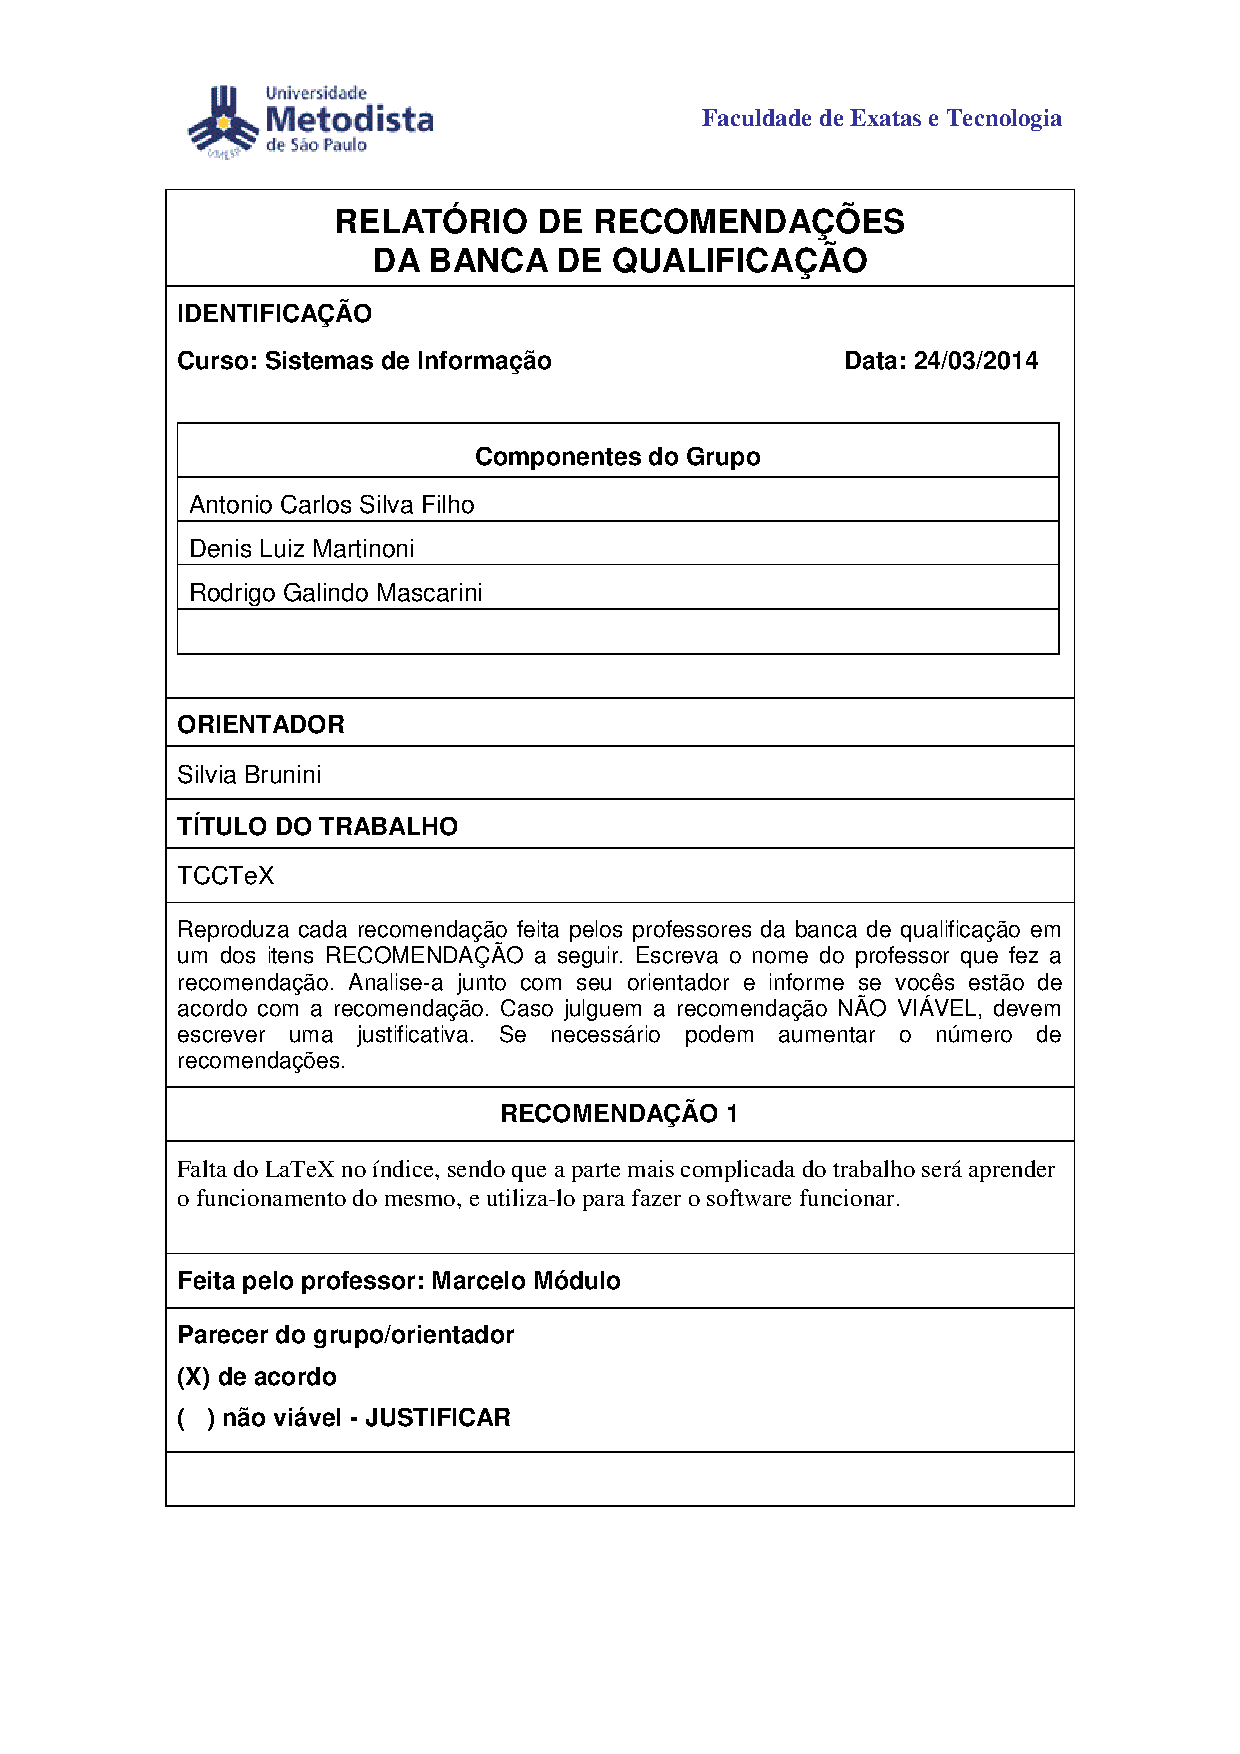
\includepdf[pages=-,pagecommand={},offset=0 -30,templatesize={145mm}{210mm}]{anexo/RRBQ.pdf}


%\include{apendices/apendice}
%Apendices - fim

\nocite{*}
%Bibliografia - Não Implementado
\bibliographystyle{abnt-alf}
\bibliography{biblio}
%Bibliografia - fim


\end{document}